\documentclass[twoside]{book}

% Packages required by doxygen
\usepackage{fixltx2e}
\usepackage{calc}
\usepackage{doxygen}
\usepackage[export]{adjustbox} % also loads graphicx
\usepackage{graphicx}
\usepackage[utf8]{inputenc}
\usepackage{makeidx}
\usepackage{multicol}
\usepackage{multirow}
\PassOptionsToPackage{warn}{textcomp}
\usepackage{textcomp}
\usepackage[nointegrals]{wasysym}
\usepackage[table]{xcolor}

% Font selection
\usepackage[T1]{fontenc}
\usepackage[scaled=.90]{helvet}
\usepackage{courier}
\usepackage{amssymb}
\usepackage{sectsty}
\renewcommand{\familydefault}{\sfdefault}
\allsectionsfont{%
  \fontseries{bc}\selectfont%
  \color{darkgray}%
}
\renewcommand{\DoxyLabelFont}{%
  \fontseries{bc}\selectfont%
  \color{darkgray}%
}
\newcommand{\+}{\discretionary{\mbox{\scriptsize$\hookleftarrow$}}{}{}}

% Page & text layout
\usepackage{geometry}
\geometry{%
  a4paper,%
  top=2.5cm,%
  bottom=2.5cm,%
  left=2.5cm,%
  right=2.5cm%
}
\tolerance=750
\hfuzz=15pt
\hbadness=750
\setlength{\emergencystretch}{15pt}
\setlength{\parindent}{0cm}
\setlength{\parskip}{3ex plus 2ex minus 2ex}
\makeatletter
\renewcommand{\paragraph}{%
  \@startsection{paragraph}{4}{0ex}{-1.0ex}{1.0ex}{%
    \normalfont\normalsize\bfseries\SS@parafont%
  }%
}
\renewcommand{\subparagraph}{%
  \@startsection{subparagraph}{5}{0ex}{-1.0ex}{1.0ex}{%
    \normalfont\normalsize\bfseries\SS@subparafont%
  }%
}
\makeatother

% Headers & footers
\usepackage{fancyhdr}
\pagestyle{fancyplain}
\fancyhead[LE]{\fancyplain{}{\bfseries\thepage}}
\fancyhead[CE]{\fancyplain{}{}}
\fancyhead[RE]{\fancyplain{}{\bfseries\leftmark}}
\fancyhead[LO]{\fancyplain{}{\bfseries\rightmark}}
\fancyhead[CO]{\fancyplain{}{}}
\fancyhead[RO]{\fancyplain{}{\bfseries\thepage}}
\fancyfoot[LE]{\fancyplain{}{}}
\fancyfoot[CE]{\fancyplain{}{}}
\fancyfoot[RE]{\fancyplain{}{\bfseries\scriptsize Generated by Doxygen }}
\fancyfoot[LO]{\fancyplain{}{\bfseries\scriptsize Generated by Doxygen }}
\fancyfoot[CO]{\fancyplain{}{}}
\fancyfoot[RO]{\fancyplain{}{}}
\renewcommand{\footrulewidth}{0.4pt}
\renewcommand{\chaptermark}[1]{%
  \markboth{#1}{}%
}
\renewcommand{\sectionmark}[1]{%
  \markright{\thesection\ #1}%
}

% Indices & bibliography
\usepackage{natbib}
\usepackage[titles]{tocloft}
\setcounter{tocdepth}{3}
\setcounter{secnumdepth}{5}
\makeindex

% Hyperlinks (required, but should be loaded last)
\usepackage{ifpdf}
\ifpdf
  \usepackage[pdftex,pagebackref=true]{hyperref}
\else
  \usepackage[ps2pdf,pagebackref=true]{hyperref}
\fi
\hypersetup{%
  colorlinks=true,%
  linkcolor=blue,%
  citecolor=blue,%
  unicode%
}

% Custom commands
\newcommand{\clearemptydoublepage}{%
  \newpage{\pagestyle{empty}\cleardoublepage}%
}

\usepackage{caption}
\captionsetup{labelsep=space,justification=centering,font={bf},singlelinecheck=off,skip=4pt,position=top}

%===== C O N T E N T S =====

\begin{document}

% Titlepage & ToC
\hypersetup{pageanchor=false,
             bookmarksnumbered=true,
             pdfencoding=unicode
            }
\pagenumbering{alph}
\begin{titlepage}
\vspace*{7cm}
\begin{center}%
{\Large kpi\+Web\+Mvc }\\
\vspace*{1cm}
{\large Generated by Doxygen 1.8.13}\\
\end{center}
\end{titlepage}
\clearemptydoublepage
\pagenumbering{roman}
\tableofcontents
\clearemptydoublepage
\pagenumbering{arabic}
\hypersetup{pageanchor=true}

%--- Begin generated contents ---
\chapter{Namespace Index}
\section{Namespace List}
Here is a list of all documented namespaces with brief descriptions\+:\begin{DoxyCompactList}
\item\contentsline{section}{\hyperlink{namespacekpi_mvc_api}{kpi\+Mvc\+Api} }{\pageref{namespacekpi_mvc_api}}{}
\item\contentsline{section}{\hyperlink{namespacekpi_mvc_api_1_1_controllers}{kpi\+Mvc\+Api.\+Controllers} }{\pageref{namespacekpi_mvc_api_1_1_controllers}}{}
\item\contentsline{section}{\hyperlink{namespacekpi_mvc_api_1_1_data_transfer_objects}{kpi\+Mvc\+Api.\+Data\+Transfer\+Objects} }{\pageref{namespacekpi_mvc_api_1_1_data_transfer_objects}}{}
\item\contentsline{section}{\hyperlink{namespacekpi_mvc_api_1_1_models}{kpi\+Mvc\+Api.\+Models} }{\pageref{namespacekpi_mvc_api_1_1_models}}{}
\end{DoxyCompactList}

\chapter{Hierarchical Index}
\section{Class Hierarchy}
This inheritance list is sorted roughly, but not completely, alphabetically\+:\begin{DoxyCompactList}
\item Api\+Controller\begin{DoxyCompactList}
\item \contentsline{section}{kpi\+Mvc\+Api.\+Controllers.\+Kpidata\+Controller}{\pageref{classkpi_mvc_api_1_1_controllers_1_1_kpidata_controller}}{}
\item \contentsline{section}{kpi\+Mvc\+Api.\+Controllers.\+Kpidata\+Controller}{\pageref{classkpi_mvc_api_1_1_controllers_1_1_kpidata_controller}}{}
\end{DoxyCompactList}
\item Controller\begin{DoxyCompactList}
\item \contentsline{section}{kpi\+Mvc\+Api.\+Controllers.\+Export\+Controller}{\pageref{classkpi_mvc_api_1_1_controllers_1_1_export_controller}}{}
\item \contentsline{section}{kpi\+Mvc\+Api.\+Controllers.\+Export\+Controller}{\pageref{classkpi_mvc_api_1_1_controllers_1_1_export_controller}}{}
\item \contentsline{section}{kpi\+Mvc\+Api.\+Controllers.\+Home\+Controller}{\pageref{classkpi_mvc_api_1_1_controllers_1_1_home_controller}}{}
\item \contentsline{section}{kpi\+Mvc\+Api.\+Controllers.\+Home\+Controller}{\pageref{classkpi_mvc_api_1_1_controllers_1_1_home_controller}}{}
\end{DoxyCompactList}
\item \contentsline{section}{kpi\+Mvc\+Api.\+Data\+Transfer\+Objects.\+Data\+Dto}{\pageref{classkpi_mvc_api_1_1_data_transfer_objects_1_1_data_dto}}{}
\begin{DoxyCompactList}
\item \contentsline{section}{kpi\+Mvc\+Api.\+Data\+Transfer\+Objects.\+Delivery\+Data\+Dto}{\pageref{classkpi_mvc_api_1_1_data_transfer_objects_1_1_delivery_data_dto}}{}
\item \contentsline{section}{kpi\+Mvc\+Api.\+Data\+Transfer\+Objects.\+Delivery\+Data\+Dto}{\pageref{classkpi_mvc_api_1_1_data_transfer_objects_1_1_delivery_data_dto}}{}
\item \contentsline{section}{kpi\+Mvc\+Api.\+Data\+Transfer\+Objects.\+Kvp\+Data\+Dto}{\pageref{classkpi_mvc_api_1_1_data_transfer_objects_1_1_kvp_data_dto}}{}
\item \contentsline{section}{kpi\+Mvc\+Api.\+Data\+Transfer\+Objects.\+Kvp\+Data\+Dto}{\pageref{classkpi_mvc_api_1_1_data_transfer_objects_1_1_kvp_data_dto}}{}
\item \contentsline{section}{kpi\+Mvc\+Api.\+Data\+Transfer\+Objects.\+Production\+Data\+Dto}{\pageref{classkpi_mvc_api_1_1_data_transfer_objects_1_1_production_data_dto}}{}
\item \contentsline{section}{kpi\+Mvc\+Api.\+Data\+Transfer\+Objects.\+Production\+Data\+Dto}{\pageref{classkpi_mvc_api_1_1_data_transfer_objects_1_1_production_data_dto}}{}
\end{DoxyCompactList}
\item \contentsline{section}{kpi\+Mvc\+Api.\+Data\+Transfer\+Objects.\+Data\+Dto\+Rs}{\pageref{classkpi_mvc_api_1_1_data_transfer_objects_1_1_data_dto_rs}}{}
\begin{DoxyCompactList}
\item \contentsline{section}{kpi\+Mvc\+Api.\+Data\+Transfer\+Objects.\+Delivery\+Data\+Dto\+Rs}{\pageref{classkpi_mvc_api_1_1_data_transfer_objects_1_1_delivery_data_dto_rs}}{}
\item \contentsline{section}{kpi\+Mvc\+Api.\+Data\+Transfer\+Objects.\+Delivery\+Data\+Dto\+Rs}{\pageref{classkpi_mvc_api_1_1_data_transfer_objects_1_1_delivery_data_dto_rs}}{}
\item \contentsline{section}{kpi\+Mvc\+Api.\+Data\+Transfer\+Objects.\+Kvp\+Data\+Dto\+Rs}{\pageref{classkpi_mvc_api_1_1_data_transfer_objects_1_1_kvp_data_dto_rs}}{}
\item \contentsline{section}{kpi\+Mvc\+Api.\+Data\+Transfer\+Objects.\+Kvp\+Data\+Dto\+Rs}{\pageref{classkpi_mvc_api_1_1_data_transfer_objects_1_1_kvp_data_dto_rs}}{}
\item \contentsline{section}{kpi\+Mvc\+Api.\+Data\+Transfer\+Objects.\+Production\+Data\+Dto\+Rs}{\pageref{classkpi_mvc_api_1_1_data_transfer_objects_1_1_production_data_dto_rs}}{}
\item \contentsline{section}{kpi\+Mvc\+Api.\+Data\+Transfer\+Objects.\+Production\+Data\+Dto\+Rs}{\pageref{classkpi_mvc_api_1_1_data_transfer_objects_1_1_production_data_dto_rs}}{}
\end{DoxyCompactList}
\item Db\+Context\begin{DoxyCompactList}
\item \contentsline{section}{kpi\+Mvc\+Api.\+Models.\+kpidb\+Entities1}{\pageref{classkpi_mvc_api_1_1_models_1_1kpidb_entities1}}{}
\item \contentsline{section}{kpi\+Mvc\+Api.\+Models.\+kpidb\+Entities1}{\pageref{classkpi_mvc_api_1_1_models_1_1kpidb_entities1}}{}
\end{DoxyCompactList}
\item \contentsline{section}{kpi\+Mvc\+Api.\+Models.\+e\+Country}{\pageref{classkpi_mvc_api_1_1_models_1_1e_country}}{}
\item \contentsline{section}{kpi\+Mvc\+Api.\+Models.\+e\+Delivery}{\pageref{classkpi_mvc_api_1_1_models_1_1e_delivery}}{}
\item \contentsline{section}{kpi\+Mvc\+Api.\+Models.\+e\+Kvp}{\pageref{classkpi_mvc_api_1_1_models_1_1e_kvp}}{}
\item \contentsline{section}{kpi\+Mvc\+Api.\+Models.\+e\+Kvp\+Class}{\pageref{classkpi_mvc_api_1_1_models_1_1e_kvp_class}}{}
\item \contentsline{section}{kpi\+Mvc\+Api.\+Models.\+e\+Kvp\+State}{\pageref{classkpi_mvc_api_1_1_models_1_1e_kvp_state}}{}
\item \contentsline{section}{kpi\+Mvc\+Api.\+Models.\+e\+Pcb\+Class}{\pageref{classkpi_mvc_api_1_1_models_1_1e_pcb_class}}{}
\item \contentsline{section}{kpi\+Mvc\+Api.\+Models.\+e\+Pcb\+Daily}{\pageref{classkpi_mvc_api_1_1_models_1_1e_pcb_daily}}{}
\item \contentsline{section}{kpi\+Mvc\+Api.\+Models.\+e\+Pcb\+Generation}{\pageref{classkpi_mvc_api_1_1_models_1_1e_pcb_generation}}{}
\item Http\+Application\begin{DoxyCompactList}
\item \contentsline{section}{kpi\+Mvc\+Api.\+Global}{\pageref{classkpi_mvc_api_1_1_global}}{}
\item \contentsline{section}{kpi\+Mvc\+Api.\+Global}{\pageref{classkpi_mvc_api_1_1_global}}{}
\end{DoxyCompactList}
\item \contentsline{section}{kpi\+Mvc\+Api.\+Route\+Config}{\pageref{classkpi_mvc_api_1_1_route_config}}{}
\end{DoxyCompactList}

\chapter{Class Index}
\section{Class List}
Here are the classes, structs, unions and interfaces with brief descriptions\+:\begin{DoxyCompactList}
\item\contentsline{section}{\hyperlink{classkpi_mvc_api_1_1_data_transfer_objects_1_1_data_dto}{kpi\+Mvc\+Api.\+Data\+Transfer\+Objects.\+Data\+Dto} }{\pageref{classkpi_mvc_api_1_1_data_transfer_objects_1_1_data_dto}}{}
\item\contentsline{section}{\hyperlink{classkpi_mvc_api_1_1_data_transfer_objects_1_1_data_dto_rs}{kpi\+Mvc\+Api.\+Data\+Transfer\+Objects.\+Data\+Dto\+Rs} }{\pageref{classkpi_mvc_api_1_1_data_transfer_objects_1_1_data_dto_rs}}{}
\item\contentsline{section}{\hyperlink{classkpi_mvc_api_1_1_data_transfer_objects_1_1_delivery_data_dto}{kpi\+Mvc\+Api.\+Data\+Transfer\+Objects.\+Delivery\+Data\+Dto} }{\pageref{classkpi_mvc_api_1_1_data_transfer_objects_1_1_delivery_data_dto}}{}
\item\contentsline{section}{\hyperlink{classkpi_mvc_api_1_1_data_transfer_objects_1_1_delivery_data_dto_rs}{kpi\+Mvc\+Api.\+Data\+Transfer\+Objects.\+Delivery\+Data\+Dto\+Rs} }{\pageref{classkpi_mvc_api_1_1_data_transfer_objects_1_1_delivery_data_dto_rs}}{}
\item\contentsline{section}{\hyperlink{classkpi_mvc_api_1_1_controllers_1_1_diagramdata_controller}{kpi\+Mvc\+Api.\+Controllers.\+Diagramdata\+Controller} }{\pageref{classkpi_mvc_api_1_1_controllers_1_1_diagramdata_controller}}{}
\item\contentsline{section}{\hyperlink{classkpi_mvc_api_1_1_data_transfer_objects_1_1_diagramdata_dto}{kpi\+Mvc\+Api.\+Data\+Transfer\+Objects.\+Diagramdata\+Dto} }{\pageref{classkpi_mvc_api_1_1_data_transfer_objects_1_1_diagramdata_dto}}{}
\item\contentsline{section}{\hyperlink{classkpi_mvc_api_1_1_data_transfer_objects_1_1_diagramdata_dto_repo}{kpi\+Mvc\+Api.\+Data\+Transfer\+Objects.\+Diagramdata\+Dto\+Repo} }{\pageref{classkpi_mvc_api_1_1_data_transfer_objects_1_1_diagramdata_dto_repo}}{}
\item\contentsline{section}{\hyperlink{classkpi_mvc_api_1_1_models_1_1e_country}{kpi\+Mvc\+Api.\+Models.\+e\+Country} }{\pageref{classkpi_mvc_api_1_1_models_1_1e_country}}{}
\item\contentsline{section}{\hyperlink{classkpi_mvc_api_1_1_models_1_1e_delivery}{kpi\+Mvc\+Api.\+Models.\+e\+Delivery} }{\pageref{classkpi_mvc_api_1_1_models_1_1e_delivery}}{}
\item\contentsline{section}{\hyperlink{classkpi_mvc_api_1_1_models_1_1e_kvp}{kpi\+Mvc\+Api.\+Models.\+e\+Kvp} }{\pageref{classkpi_mvc_api_1_1_models_1_1e_kvp}}{}
\item\contentsline{section}{\hyperlink{classkpi_mvc_api_1_1_models_1_1e_kvp_class}{kpi\+Mvc\+Api.\+Models.\+e\+Kvp\+Class} }{\pageref{classkpi_mvc_api_1_1_models_1_1e_kvp_class}}{}
\item\contentsline{section}{\hyperlink{classkpi_mvc_api_1_1_models_1_1e_kvp_state}{kpi\+Mvc\+Api.\+Models.\+e\+Kvp\+State} }{\pageref{classkpi_mvc_api_1_1_models_1_1e_kvp_state}}{}
\item\contentsline{section}{\hyperlink{classkpi_mvc_api_1_1_models_1_1e_pcb_class}{kpi\+Mvc\+Api.\+Models.\+e\+Pcb\+Class} }{\pageref{classkpi_mvc_api_1_1_models_1_1e_pcb_class}}{}
\item\contentsline{section}{\hyperlink{classkpi_mvc_api_1_1_models_1_1e_pcb_daily}{kpi\+Mvc\+Api.\+Models.\+e\+Pcb\+Daily} }{\pageref{classkpi_mvc_api_1_1_models_1_1e_pcb_daily}}{}
\item\contentsline{section}{\hyperlink{classkpi_mvc_api_1_1_models_1_1e_pcb_generation}{kpi\+Mvc\+Api.\+Models.\+e\+Pcb\+Generation} }{\pageref{classkpi_mvc_api_1_1_models_1_1e_pcb_generation}}{}
\item\contentsline{section}{\hyperlink{classkpi_mvc_api_1_1_controllers_1_1_export_controller}{kpi\+Mvc\+Api.\+Controllers.\+Export\+Controller} \\*Der Exportkontroller stellt den alle Dienste zur exportierung von Files zur Verfügung. }{\pageref{classkpi_mvc_api_1_1_controllers_1_1_export_controller}}{}
\item\contentsline{section}{\hyperlink{classkpi_mvc_api_1_1_global}{kpi\+Mvc\+Api.\+Global} }{\pageref{classkpi_mvc_api_1_1_global}}{}
\item\contentsline{section}{\hyperlink{classkpi_mvc_api_1_1_controllers_1_1_home_controller}{kpi\+Mvc\+Api.\+Controllers.\+Home\+Controller} \\*Webseite Controller Setllt die Views und die Partaialviews bereit }{\pageref{classkpi_mvc_api_1_1_controllers_1_1_home_controller}}{}
\item\contentsline{section}{\hyperlink{classkpi_mvc_api_1_1_controllers_1_1_kpidata_controller}{kpi\+Mvc\+Api.\+Controllers.\+Kpidata\+Controller} }{\pageref{classkpi_mvc_api_1_1_controllers_1_1_kpidata_controller}}{}
\item\contentsline{section}{\hyperlink{classkpi_mvc_api_1_1_models_1_1kpidb_entities1}{kpi\+Mvc\+Api.\+Models.\+kpidb\+Entities1} }{\pageref{classkpi_mvc_api_1_1_models_1_1kpidb_entities1}}{}
\item\contentsline{section}{\hyperlink{classkpi_mvc_api_1_1_data_transfer_objects_1_1_kvp_data_dto}{kpi\+Mvc\+Api.\+Data\+Transfer\+Objects.\+Kvp\+Data\+Dto} }{\pageref{classkpi_mvc_api_1_1_data_transfer_objects_1_1_kvp_data_dto}}{}
\item\contentsline{section}{\hyperlink{classkpi_mvc_api_1_1_data_transfer_objects_1_1_kvp_data_dto_rs}{kpi\+Mvc\+Api.\+Data\+Transfer\+Objects.\+Kvp\+Data\+Dto\+Rs} }{\pageref{classkpi_mvc_api_1_1_data_transfer_objects_1_1_kvp_data_dto_rs}}{}
\item\contentsline{section}{\hyperlink{classkpi_mvc_api_1_1_data_transfer_objects_1_1_kvp_dto}{kpi\+Mvc\+Api.\+Data\+Transfer\+Objects.\+Kvp\+Dto} }{\pageref{classkpi_mvc_api_1_1_data_transfer_objects_1_1_kvp_dto}}{}
\item\contentsline{section}{\hyperlink{classkpi_mvc_api_1_1_data_transfer_objects_1_1_production_data_dto}{kpi\+Mvc\+Api.\+Data\+Transfer\+Objects.\+Production\+Data\+Dto} }{\pageref{classkpi_mvc_api_1_1_data_transfer_objects_1_1_production_data_dto}}{}
\item\contentsline{section}{\hyperlink{classkpi_mvc_api_1_1_data_transfer_objects_1_1_production_data_dto_rs}{kpi\+Mvc\+Api.\+Data\+Transfer\+Objects.\+Production\+Data\+Dto\+Rs} }{\pageref{classkpi_mvc_api_1_1_data_transfer_objects_1_1_production_data_dto_rs}}{}
\item\contentsline{section}{\hyperlink{classkpi_mvc_api_1_1_route_config}{kpi\+Mvc\+Api.\+Route\+Config} }{\pageref{classkpi_mvc_api_1_1_route_config}}{}
\item\contentsline{section}{\hyperlink{classkpi_mvc_api_1_1_models_1_1_site_model}{kpi\+Mvc\+Api.\+Models.\+Site\+Model} }{\pageref{classkpi_mvc_api_1_1_models_1_1_site_model}}{}
\end{DoxyCompactList}

\chapter{Namespace Documentation}
\hypertarget{namespacekpi_mvc_api}{}\section{kpi\+Mvc\+Api Namespace Reference}
\label{namespacekpi_mvc_api}\index{kpi\+Mvc\+Api@{kpi\+Mvc\+Api}}
\subsection*{Namespaces}
\begin{DoxyCompactItemize}
\item 
namespace \hyperlink{namespacekpi_mvc_api_1_1_controllers}{Controllers}
\begin{DoxyCompactList}\small\item\em Implementiert die Controller der Dashboard Api \end{DoxyCompactList}\end{DoxyCompactItemize}
\subsection*{Classes}
\begin{DoxyCompactItemize}
\item 
class \hyperlink{classkpi_mvc_api_1_1_global}{Global}
\item 
class \hyperlink{classkpi_mvc_api_1_1_route_config}{Route\+Config}
\item 
class {\bfseries Web\+Api\+Config}
\end{DoxyCompactItemize}

\hypertarget{namespacekpi_mvc_api_1_1_controllers}{}\section{kpi\+Mvc\+Api.\+Controllers Namespace Reference}
\label{namespacekpi_mvc_api_1_1_controllers}\index{kpi\+Mvc\+Api.\+Controllers@{kpi\+Mvc\+Api.\+Controllers}}


Implementiert die Controller der Dashboard Api  


\subsection*{Classes}
\begin{DoxyCompactItemize}
\item 
class \hyperlink{classkpi_mvc_api_1_1_controllers_1_1_diagramdata_controller}{Diagramdata\+Controller}
\item 
class \hyperlink{classkpi_mvc_api_1_1_controllers_1_1_export_controller}{Export\+Controller}
\begin{DoxyCompactList}\small\item\em Der Exportkontroller stellt den alle Dienste zur exportierung von Files zur Verfügung. \end{DoxyCompactList}\item 
class \hyperlink{classkpi_mvc_api_1_1_controllers_1_1_home_controller}{Home\+Controller}
\item 
class \hyperlink{classkpi_mvc_api_1_1_controllers_1_1_kpidata_controller}{Kpidata\+Controller}
\end{DoxyCompactItemize}


\subsection{Detailed Description}
Implementiert die Controller der Dashboard Api 


\hypertarget{namespacekpi_mvc_api_1_1_data_transfer_objects}{}\section{kpi\+Mvc\+Api.\+Data\+Transfer\+Objects Namespace Reference}
\label{namespacekpi_mvc_api_1_1_data_transfer_objects}\index{kpi\+Mvc\+Api.\+Data\+Transfer\+Objects@{kpi\+Mvc\+Api.\+Data\+Transfer\+Objects}}
\subsection*{Classes}
\begin{DoxyCompactItemize}
\item 
class \hyperlink{classkpi_mvc_api_1_1_data_transfer_objects_1_1_delivery_data_dto}{Delivery\+Data\+Dto}
\item 
class \hyperlink{classkpi_mvc_api_1_1_data_transfer_objects_1_1_diagramdata_dto}{Diagramdata\+Dto}
\item 
class \hyperlink{classkpi_mvc_api_1_1_data_transfer_objects_1_1_diagramdata_dto_repo}{Diagramdata\+Dto\+Repo}
\item 
class \hyperlink{classkpi_mvc_api_1_1_data_transfer_objects_1_1_kvp_data_dto}{Kvp\+Data\+Dto}
\item 
class \hyperlink{classkpi_mvc_api_1_1_data_transfer_objects_1_1_kvp_data_dto_rs}{Kvp\+Data\+Dto\+Rs}
\item 
class \hyperlink{classkpi_mvc_api_1_1_data_transfer_objects_1_1_production_data_dto}{Production\+Data\+Dto}
\item 
class \hyperlink{classkpi_mvc_api_1_1_data_transfer_objects_1_1_production_data_dto_rs}{Production\+Data\+Dto\+Rs}
\end{DoxyCompactItemize}

\hypertarget{namespacekpi_mvc_api_1_1_models}{}\section{kpi\+Mvc\+Api.\+Models Namespace Reference}
\label{namespacekpi_mvc_api_1_1_models}\index{kpi\+Mvc\+Api.\+Models@{kpi\+Mvc\+Api.\+Models}}
\subsection*{Classes}
\begin{DoxyCompactItemize}
\item 
class \hyperlink{classkpi_mvc_api_1_1_models_1_1e_country}{e\+Country}
\item 
class \hyperlink{classkpi_mvc_api_1_1_models_1_1e_delivery}{e\+Delivery}
\item 
class \hyperlink{classkpi_mvc_api_1_1_models_1_1e_kvp}{e\+Kvp}
\item 
class \hyperlink{classkpi_mvc_api_1_1_models_1_1e_kvp_class}{e\+Kvp\+Class}
\item 
class \hyperlink{classkpi_mvc_api_1_1_models_1_1e_kvp_state}{e\+Kvp\+State}
\item 
class \hyperlink{classkpi_mvc_api_1_1_models_1_1e_pcb_class}{e\+Pcb\+Class}
\item 
class \hyperlink{classkpi_mvc_api_1_1_models_1_1e_pcb_daily}{e\+Pcb\+Daily}
\item 
class \hyperlink{classkpi_mvc_api_1_1_models_1_1e_pcb_generation}{e\+Pcb\+Generation}
\item 
class \hyperlink{classkpi_mvc_api_1_1_models_1_1kpidb_entities1}{kpidb\+Entities1}
\end{DoxyCompactItemize}

\chapter{Class Documentation}
\hypertarget{classkpi_mvc_api_1_1_data_transfer_objects_1_1_delivery_dto}{}\section{kpi\+Mvc\+Api.\+Data\+Transfer\+Objects.\+Delivery\+Dto Class Reference}
\label{classkpi_mvc_api_1_1_data_transfer_objects_1_1_delivery_dto}\index{kpi\+Mvc\+Api.\+Data\+Transfer\+Objects.\+Delivery\+Dto@{kpi\+Mvc\+Api.\+Data\+Transfer\+Objects.\+Delivery\+Dto}}
\subsection*{Properties}
\begin{DoxyCompactItemize}
\item 
\mbox{\Hypertarget{classkpi_mvc_api_1_1_data_transfer_objects_1_1_delivery_dto_abfa55f92ce2eb311f109bbf00adf0fae}\label{classkpi_mvc_api_1_1_data_transfer_objects_1_1_delivery_dto_abfa55f92ce2eb311f109bbf00adf0fae}} 
int {\bfseries Delivery\+Id}\hspace{0.3cm}{\ttfamily  \mbox{[}get, set\mbox{]}}
\item 
\mbox{\Hypertarget{classkpi_mvc_api_1_1_data_transfer_objects_1_1_delivery_dto_a55b63a4dd02ad1ac985c5e14c074f844}\label{classkpi_mvc_api_1_1_data_transfer_objects_1_1_delivery_dto_a55b63a4dd02ad1ac985c5e14c074f844}} 
Date\+Time {\bfseries Order\+Date}\hspace{0.3cm}{\ttfamily  \mbox{[}get, set\mbox{]}}
\item 
\mbox{\Hypertarget{classkpi_mvc_api_1_1_data_transfer_objects_1_1_delivery_dto_a8aee4a265f39d1065f7ce062a9d612fb}\label{classkpi_mvc_api_1_1_data_transfer_objects_1_1_delivery_dto_a8aee4a265f39d1065f7ce062a9d612fb}} 
int {\bfseries Ordered\+Pc}\hspace{0.3cm}{\ttfamily  \mbox{[}get, set\mbox{]}}
\item 
\mbox{\Hypertarget{classkpi_mvc_api_1_1_data_transfer_objects_1_1_delivery_dto_a307da11b2af0c2faa34c8306bd9aae5b}\label{classkpi_mvc_api_1_1_data_transfer_objects_1_1_delivery_dto_a307da11b2af0c2faa34c8306bd9aae5b}} 
int {\bfseries Delivered\+Pc}\hspace{0.3cm}{\ttfamily  \mbox{[}get, set\mbox{]}}
\item 
\mbox{\Hypertarget{classkpi_mvc_api_1_1_data_transfer_objects_1_1_delivery_dto_aa15e3fa45b13f2d466ec060e65c3932d}\label{classkpi_mvc_api_1_1_data_transfer_objects_1_1_delivery_dto_aa15e3fa45b13f2d466ec060e65c3932d}} 
int {\bfseries Notdelivered\+Pc}\hspace{0.3cm}{\ttfamily  \mbox{[}get, set\mbox{]}}
\item 
\mbox{\Hypertarget{classkpi_mvc_api_1_1_data_transfer_objects_1_1_delivery_dto_a74702ba97da373adab874c2dc6422bc7}\label{classkpi_mvc_api_1_1_data_transfer_objects_1_1_delivery_dto_a74702ba97da373adab874c2dc6422bc7}} 
float {\bfseries Notdelivered\+Rel}\hspace{0.3cm}{\ttfamily  \mbox{[}get, set\mbox{]}}
\item 
\mbox{\Hypertarget{classkpi_mvc_api_1_1_data_transfer_objects_1_1_delivery_dto_a96cbf3036055a923f4def0d846905af7}\label{classkpi_mvc_api_1_1_data_transfer_objects_1_1_delivery_dto_a96cbf3036055a923f4def0d846905af7}} 
int {\bfseries Country\+Id}\hspace{0.3cm}{\ttfamily  \mbox{[}get, set\mbox{]}}
\item 
\mbox{\Hypertarget{classkpi_mvc_api_1_1_data_transfer_objects_1_1_delivery_dto_a5ece3ff3a399d3b2baff4fccef29cdc1}\label{classkpi_mvc_api_1_1_data_transfer_objects_1_1_delivery_dto_a5ece3ff3a399d3b2baff4fccef29cdc1}} 
string {\bfseries Country\+Name}\hspace{0.3cm}{\ttfamily  \mbox{[}get, set\mbox{]}}
\end{DoxyCompactItemize}


The documentation for this class was generated from the following file\+:\begin{DoxyCompactItemize}
\item 
C\+:/\+Users/i00202128/\+Source/\+Repos/kpi\+Web\+Mvc/kpi\+Mvc/kpi\+Mvc\+Api/\+Data\+Transfer\+Objects/Delivery\+Dto.\+cs\end{DoxyCompactItemize}

\hypertarget{classkpi_mvc_api_1_1_controllers_1_1_diagramdata_controller}{}\section{kpi\+Mvc\+Api.\+Controllers.\+Diagramdata\+Controller Class Reference}
\label{classkpi_mvc_api_1_1_controllers_1_1_diagramdata_controller}\index{kpi\+Mvc\+Api.\+Controllers.\+Diagramdata\+Controller@{kpi\+Mvc\+Api.\+Controllers.\+Diagramdata\+Controller}}
Inheritance diagram for kpi\+Mvc\+Api.\+Controllers.\+Diagramdata\+Controller\+:\begin{figure}[H]
\begin{center}
\leavevmode
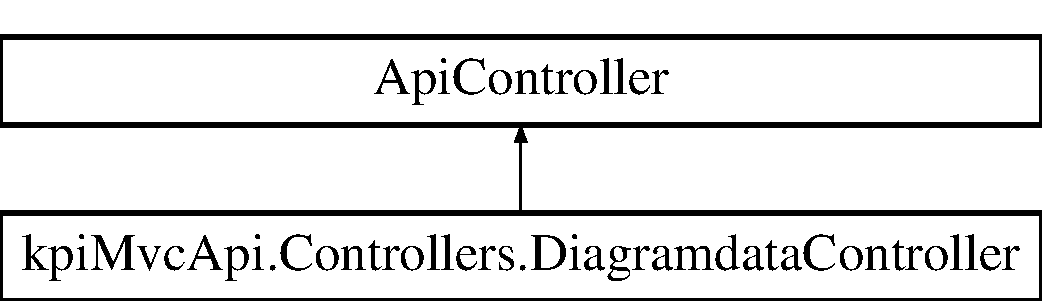
\includegraphics[height=2.000000cm]{classkpi_mvc_api_1_1_controllers_1_1_diagramdata_controller}
\end{center}
\end{figure}
\subsection*{Public Member Functions}
\begin{DoxyCompactItemize}
\item 
\mbox{\Hypertarget{classkpi_mvc_api_1_1_controllers_1_1_diagramdata_controller_a1e2708509e980e3e6eeb52477826dc87}\label{classkpi_mvc_api_1_1_controllers_1_1_diagramdata_controller_a1e2708509e980e3e6eeb52477826dc87}} 
I\+Enumerable$<$ \hyperlink{classkpi_mvc_api_1_1_data_transfer_objects_1_1_diagramdata_dto}{Diagramdata\+Dto} $>$ {\bfseries Get} (int? diagram)
\end{DoxyCompactItemize}


The documentation for this class was generated from the following file\+:\begin{DoxyCompactItemize}
\item 
C\+:/\+Users/\+Ulysses/\+Documents/01\+\_\+\+Study\+Fhnw/815\+\_\+veri/kpi\+Web\+Mvc/kpi\+Mvc/kpi\+Mvc\+Api/obj/\+Debug/\+Package/\+Package\+Tmp/\+Controllers/Diagramdata\+Controller.\+cs\end{DoxyCompactItemize}

\hypertarget{classkpi_mvc_api_1_1_data_transfer_objects_1_1_diagramdata_dto}{}\section{kpi\+Mvc\+Api.\+Data\+Transfer\+Objects.\+Diagramdata\+Dto Class Reference}
\label{classkpi_mvc_api_1_1_data_transfer_objects_1_1_diagramdata_dto}\index{kpi\+Mvc\+Api.\+Data\+Transfer\+Objects.\+Diagramdata\+Dto@{kpi\+Mvc\+Api.\+Data\+Transfer\+Objects.\+Diagramdata\+Dto}}
\subsection*{Properties}
\begin{DoxyCompactItemize}
\item 
\mbox{\Hypertarget{classkpi_mvc_api_1_1_data_transfer_objects_1_1_diagramdata_dto_a2f1c78c25410b5d89692f417c0099414}\label{classkpi_mvc_api_1_1_data_transfer_objects_1_1_diagramdata_dto_a2f1c78c25410b5d89692f417c0099414}} 
int {\bfseries Diagram\+Data\+Id}\hspace{0.3cm}{\ttfamily  \mbox{[}get, set\mbox{]}}
\item 
\mbox{\Hypertarget{classkpi_mvc_api_1_1_data_transfer_objects_1_1_diagramdata_dto_a5cb8e04b29f5c657d4185b426eeb84da}\label{classkpi_mvc_api_1_1_data_transfer_objects_1_1_diagramdata_dto_a5cb8e04b29f5c657d4185b426eeb84da}} 
string {\bfseries Diagram\+Data\+Label}\hspace{0.3cm}{\ttfamily  \mbox{[}get, set\mbox{]}}
\item 
\mbox{\Hypertarget{classkpi_mvc_api_1_1_data_transfer_objects_1_1_diagramdata_dto_a4163112f5037d60673ac0d3ef3603fc8}\label{classkpi_mvc_api_1_1_data_transfer_objects_1_1_diagramdata_dto_a4163112f5037d60673ac0d3ef3603fc8}} 
string {\bfseries Diagram\+Data}\hspace{0.3cm}{\ttfamily  \mbox{[}get, set\mbox{]}}
\end{DoxyCompactItemize}


The documentation for this class was generated from the following file\+:\begin{DoxyCompactItemize}
\item 
C\+:/\+Users/\+Ulysses/\+Documents/01\+\_\+\+Study\+Fhnw/815\+\_\+veri/kpi\+Web\+Mvc/kpi\+Mvc/kpi\+Mvc\+Api/obj/\+Debug/\+Package/\+Package\+Tmp/\+Data\+Transfer\+Objects/Diagramdata\+Dto.\+cs\end{DoxyCompactItemize}

\hypertarget{classkpi_mvc_api_1_1_data_transfer_objects_1_1_diagramdata_dto_repo}{}\section{kpi\+Mvc\+Api.\+Data\+Transfer\+Objects.\+Diagramdata\+Dto\+Repo Class Reference}
\label{classkpi_mvc_api_1_1_data_transfer_objects_1_1_diagramdata_dto_repo}\index{kpi\+Mvc\+Api.\+Data\+Transfer\+Objects.\+Diagramdata\+Dto\+Repo@{kpi\+Mvc\+Api.\+Data\+Transfer\+Objects.\+Diagramdata\+Dto\+Repo}}
\subsection*{Public Types}
\begin{DoxyCompactItemize}
\item 
\mbox{\Hypertarget{classkpi_mvc_api_1_1_data_transfer_objects_1_1_diagramdata_dto_repo_a58bbabee43b0cec73f86ae00072a5ba6}\label{classkpi_mvc_api_1_1_data_transfer_objects_1_1_diagramdata_dto_repo_a58bbabee43b0cec73f86ae00072a5ba6}} 
enum {\bfseries charts} \{ {\bfseries Testchart} = 1, 
{\bfseries Debugchart}
 \}
\end{DoxyCompactItemize}
\subsection*{Public Member Functions}
\begin{DoxyCompactItemize}
\item 
\mbox{\Hypertarget{classkpi_mvc_api_1_1_data_transfer_objects_1_1_diagramdata_dto_repo_a20acbfa7c0cc330f40ea80fae3a8ba87}\label{classkpi_mvc_api_1_1_data_transfer_objects_1_1_diagramdata_dto_repo_a20acbfa7c0cc330f40ea80fae3a8ba87}} 
List$<$ \hyperlink{classkpi_mvc_api_1_1_data_transfer_objects_1_1_diagramdata_dto}{Diagramdata\+Dto} $>$ {\bfseries gen\+Randomised\+Data} (int len)
\end{DoxyCompactItemize}
\subsection*{Properties}
\begin{DoxyCompactItemize}
\item 
\mbox{\Hypertarget{classkpi_mvc_api_1_1_data_transfer_objects_1_1_diagramdata_dto_repo_a832e84f15dc1ff02134038bf8325306d}\label{classkpi_mvc_api_1_1_data_transfer_objects_1_1_diagramdata_dto_repo_a832e84f15dc1ff02134038bf8325306d}} 
List$<$ \hyperlink{classkpi_mvc_api_1_1_data_transfer_objects_1_1_diagramdata_dto}{Diagramdata\+Dto} $>$ {\bfseries Diagram\+Data\+Repo}\hspace{0.3cm}{\ttfamily  \mbox{[}get, set\mbox{]}}
\end{DoxyCompactItemize}


The documentation for this class was generated from the following file\+:\begin{DoxyCompactItemize}
\item 
C\+:/\+Users/i00202128/\+Source/\+Repos/kpi\+Web\+Mvc/kpi\+Mvc/kpi\+Mvc\+Api/\+Data\+Transfer\+Objects/Diagramdata\+Dto\+Repo.\+cs\end{DoxyCompactItemize}

\hypertarget{classkpi_mvc_api_1_1_models_1_1e_country}{}\section{kpi\+Mvc\+Api.\+Models.\+e\+Country Class Reference}
\label{classkpi_mvc_api_1_1_models_1_1e_country}\index{kpi\+Mvc\+Api.\+Models.\+e\+Country@{kpi\+Mvc\+Api.\+Models.\+e\+Country}}
\subsection*{Properties}
\begin{DoxyCompactItemize}
\item 
\mbox{\Hypertarget{classkpi_mvc_api_1_1_models_1_1e_country_a514ea03591f2054a5542c795222acc78}\label{classkpi_mvc_api_1_1_models_1_1e_country_a514ea03591f2054a5542c795222acc78}} 
int {\bfseries country\+Id}\hspace{0.3cm}{\ttfamily  \mbox{[}get, set\mbox{]}}
\item 
\mbox{\Hypertarget{classkpi_mvc_api_1_1_models_1_1e_country_ae12d3e0cc04f926c5f18a0742da93bf1}\label{classkpi_mvc_api_1_1_models_1_1e_country_ae12d3e0cc04f926c5f18a0742da93bf1}} 
string {\bfseries country\+Name}\hspace{0.3cm}{\ttfamily  \mbox{[}get, set\mbox{]}}
\item 
\mbox{\Hypertarget{classkpi_mvc_api_1_1_models_1_1e_country_a9e3c718ad38b78b9846b0ee49e4ec77c}\label{classkpi_mvc_api_1_1_models_1_1e_country_a9e3c718ad38b78b9846b0ee49e4ec77c}} 
virtual \hyperlink{classkpi_mvc_api_1_1_models_1_1e_delivery}{e\+Delivery} {\bfseries e\+Delivery}\hspace{0.3cm}{\ttfamily  \mbox{[}get, set\mbox{]}}
\end{DoxyCompactItemize}


The documentation for this class was generated from the following file\+:\begin{DoxyCompactItemize}
\item 
C\+:/\+Users/i00202128/\+Source/\+Repos/kpi\+Web\+Mvc/kpi\+Mvc/kpi\+Mvc\+Api/\+Models/e\+Country.\+cs\end{DoxyCompactItemize}

\hypertarget{classkpi_mvc_api_1_1_models_1_1e_delivery}{}\section{kpi\+Mvc\+Api.\+Models.\+e\+Delivery Class Reference}
\label{classkpi_mvc_api_1_1_models_1_1e_delivery}\index{kpi\+Mvc\+Api.\+Models.\+e\+Delivery@{kpi\+Mvc\+Api.\+Models.\+e\+Delivery}}
\subsection*{Properties}
\begin{DoxyCompactItemize}
\item 
\mbox{\Hypertarget{classkpi_mvc_api_1_1_models_1_1e_delivery_a27d662c39ab697df7cca8ffc6bd07d56}\label{classkpi_mvc_api_1_1_models_1_1e_delivery_a27d662c39ab697df7cca8ffc6bd07d56}} 
int {\bfseries delivery\+Id}\hspace{0.3cm}{\ttfamily  \mbox{[}get, set\mbox{]}}
\item 
\mbox{\Hypertarget{classkpi_mvc_api_1_1_models_1_1e_delivery_a0fea3a43fefa66619cfe204f09af9c13}\label{classkpi_mvc_api_1_1_models_1_1e_delivery_a0fea3a43fefa66619cfe204f09af9c13}} 
System.\+Date\+Time {\bfseries order\+Date}\hspace{0.3cm}{\ttfamily  \mbox{[}get, set\mbox{]}}
\item 
\mbox{\Hypertarget{classkpi_mvc_api_1_1_models_1_1e_delivery_a7e84600c0076d7eda44d598e028c4472}\label{classkpi_mvc_api_1_1_models_1_1e_delivery_a7e84600c0076d7eda44d598e028c4472}} 
int {\bfseries ordered\+Pc}\hspace{0.3cm}{\ttfamily  \mbox{[}get, set\mbox{]}}
\item 
\mbox{\Hypertarget{classkpi_mvc_api_1_1_models_1_1e_delivery_a3361eda53db33d04571cb0d86e6a3e4c}\label{classkpi_mvc_api_1_1_models_1_1e_delivery_a3361eda53db33d04571cb0d86e6a3e4c}} 
int {\bfseries delivered\+Pc}\hspace{0.3cm}{\ttfamily  \mbox{[}get, set\mbox{]}}
\item 
\mbox{\Hypertarget{classkpi_mvc_api_1_1_models_1_1e_delivery_a926ff2a872a98cccfd72dab827a9b273}\label{classkpi_mvc_api_1_1_models_1_1e_delivery_a926ff2a872a98cccfd72dab827a9b273}} 
Nullable$<$ int $>$ {\bfseries notdelivered\+Pc}\hspace{0.3cm}{\ttfamily  \mbox{[}get, set\mbox{]}}
\item 
\mbox{\Hypertarget{classkpi_mvc_api_1_1_models_1_1e_delivery_af7ad3ae216a55ec0bb62e8fcffa3d49a}\label{classkpi_mvc_api_1_1_models_1_1e_delivery_af7ad3ae216a55ec0bb62e8fcffa3d49a}} 
int {\bfseries country\+Id}\hspace{0.3cm}{\ttfamily  \mbox{[}get, set\mbox{]}}
\item 
\mbox{\Hypertarget{classkpi_mvc_api_1_1_models_1_1e_delivery_a008a94aecbb8b3262033f8f1baaf3783}\label{classkpi_mvc_api_1_1_models_1_1e_delivery_a008a94aecbb8b3262033f8f1baaf3783}} 
Nullable$<$ int $>$ {\bfseries notdelivered\+Rel}\hspace{0.3cm}{\ttfamily  \mbox{[}get, set\mbox{]}}
\item 
\mbox{\Hypertarget{classkpi_mvc_api_1_1_models_1_1e_delivery_afa5e4760b557faeda41e1424dd2b57d4}\label{classkpi_mvc_api_1_1_models_1_1e_delivery_afa5e4760b557faeda41e1424dd2b57d4}} 
virtual \hyperlink{classkpi_mvc_api_1_1_models_1_1e_country}{e\+Country} {\bfseries e\+Country}\hspace{0.3cm}{\ttfamily  \mbox{[}get, set\mbox{]}}
\end{DoxyCompactItemize}


The documentation for this class was generated from the following file\+:\begin{DoxyCompactItemize}
\item 
C\+:/\+Users/i00202128/\+Source/\+Repos/kpi\+Web\+Mvc/kpi\+Mvc/kpi\+Mvc\+Api/\+Models/e\+Delivery.\+cs\end{DoxyCompactItemize}

\hypertarget{classkpi_mvc_api_1_1_models_1_1e_kvp}{}\section{kpi\+Mvc\+Api.\+Models.\+e\+Kvp Class Reference}
\label{classkpi_mvc_api_1_1_models_1_1e_kvp}\index{kpi\+Mvc\+Api.\+Models.\+e\+Kvp@{kpi\+Mvc\+Api.\+Models.\+e\+Kvp}}
\subsection*{Properties}
\begin{DoxyCompactItemize}
\item 
\mbox{\Hypertarget{classkpi_mvc_api_1_1_models_1_1e_kvp_a54711885ac704976abd6cdd7c73854f4}\label{classkpi_mvc_api_1_1_models_1_1e_kvp_a54711885ac704976abd6cdd7c73854f4}} 
int {\bfseries kvp\+Id}\hspace{0.3cm}{\ttfamily  \mbox{[}get, set\mbox{]}}
\item 
\mbox{\Hypertarget{classkpi_mvc_api_1_1_models_1_1e_kvp_ac7077b2c7a571312ed6e045654479530}\label{classkpi_mvc_api_1_1_models_1_1e_kvp_ac7077b2c7a571312ed6e045654479530}} 
string {\bfseries kvp\+Name}\hspace{0.3cm}{\ttfamily  \mbox{[}get, set\mbox{]}}
\item 
\mbox{\Hypertarget{classkpi_mvc_api_1_1_models_1_1e_kvp_acc1df62c2f87bb2ab5b522f189b784fc}\label{classkpi_mvc_api_1_1_models_1_1e_kvp_acc1df62c2f87bb2ab5b522f189b784fc}} 
System.\+Date\+Time {\bfseries kvp\+Date}\hspace{0.3cm}{\ttfamily  \mbox{[}get, set\mbox{]}}
\item 
\mbox{\Hypertarget{classkpi_mvc_api_1_1_models_1_1e_kvp_a89cd29a46a7e2db987eca1191bf0c7a0}\label{classkpi_mvc_api_1_1_models_1_1e_kvp_a89cd29a46a7e2db987eca1191bf0c7a0}} 
int {\bfseries kvp\+Class\+Id}\hspace{0.3cm}{\ttfamily  \mbox{[}get, set\mbox{]}}
\item 
\mbox{\Hypertarget{classkpi_mvc_api_1_1_models_1_1e_kvp_a835622d2cdae326e75fc66f396daca06}\label{classkpi_mvc_api_1_1_models_1_1e_kvp_a835622d2cdae326e75fc66f396daca06}} 
int {\bfseries kvp\+State\+Id}\hspace{0.3cm}{\ttfamily  \mbox{[}get, set\mbox{]}}
\item 
\mbox{\Hypertarget{classkpi_mvc_api_1_1_models_1_1e_kvp_a9d8ab28be21d4e0e8e511de170cc47d8}\label{classkpi_mvc_api_1_1_models_1_1e_kvp_a9d8ab28be21d4e0e8e511de170cc47d8}} 
virtual \hyperlink{classkpi_mvc_api_1_1_models_1_1e_kvp_class}{e\+Kvp\+Class} {\bfseries e\+Kvp\+Class}\hspace{0.3cm}{\ttfamily  \mbox{[}get, set\mbox{]}}
\item 
\mbox{\Hypertarget{classkpi_mvc_api_1_1_models_1_1e_kvp_a63ab869f458a5a35e6a0787a87898191}\label{classkpi_mvc_api_1_1_models_1_1e_kvp_a63ab869f458a5a35e6a0787a87898191}} 
virtual \hyperlink{classkpi_mvc_api_1_1_models_1_1e_kvp_state}{e\+Kvp\+State} {\bfseries e\+Kvp\+State}\hspace{0.3cm}{\ttfamily  \mbox{[}get, set\mbox{]}}
\end{DoxyCompactItemize}


The documentation for this class was generated from the following file\+:\begin{DoxyCompactItemize}
\item 
C\+:/\+Users/\+Ulysses/\+Documents/01\+\_\+\+Study\+Fhnw/815\+\_\+veri/kpi\+Web\+Mvc/kpi\+Mvc/kpi\+Mvc\+Api/\+Models/e\+Kvp.\+cs\end{DoxyCompactItemize}

\hypertarget{classkpi_mvc_api_1_1_models_1_1e_kvp_class}{}\section{kpi\+Mvc\+Api.\+Models.\+e\+Kvp\+Class Class Reference}
\label{classkpi_mvc_api_1_1_models_1_1e_kvp_class}\index{kpi\+Mvc\+Api.\+Models.\+e\+Kvp\+Class@{kpi\+Mvc\+Api.\+Models.\+e\+Kvp\+Class}}
\subsection*{Properties}
\begin{DoxyCompactItemize}
\item 
\mbox{\Hypertarget{classkpi_mvc_api_1_1_models_1_1e_kvp_class_a7ac3bfff016e0b0121f263fa64f37c62}\label{classkpi_mvc_api_1_1_models_1_1e_kvp_class_a7ac3bfff016e0b0121f263fa64f37c62}} 
int {\bfseries kvp\+Class\+Id}\hspace{0.3cm}{\ttfamily  \mbox{[}get, set\mbox{]}}
\item 
\mbox{\Hypertarget{classkpi_mvc_api_1_1_models_1_1e_kvp_class_aec8b691ef5964ff4debf2bce8dcb10c0}\label{classkpi_mvc_api_1_1_models_1_1e_kvp_class_aec8b691ef5964ff4debf2bce8dcb10c0}} 
string {\bfseries kvp\+Class\+Name}\hspace{0.3cm}{\ttfamily  \mbox{[}get, set\mbox{]}}
\item 
\mbox{\Hypertarget{classkpi_mvc_api_1_1_models_1_1e_kvp_class_a6e00a631be68d6e6e5a130024b0cdc9b}\label{classkpi_mvc_api_1_1_models_1_1e_kvp_class_a6e00a631be68d6e6e5a130024b0cdc9b}} 
virtual I\+Collection$<$ \hyperlink{classkpi_mvc_api_1_1_models_1_1e_kvp}{e\+Kvp} $>$ {\bfseries e\+Kvps}\hspace{0.3cm}{\ttfamily  \mbox{[}get, set\mbox{]}}
\end{DoxyCompactItemize}


The documentation for this class was generated from the following file\+:\begin{DoxyCompactItemize}
\item 
C\+:/\+Users/\+Ulysses/\+Documents/01\+\_\+\+Study\+Fhnw/815\+\_\+veri/kpi\+Web\+Mvc/kpi\+Mvc/kpi\+Mvc\+Api/\+Models/e\+Kvp\+Class.\+cs\end{DoxyCompactItemize}

\hypertarget{classkpi_mvc_api_1_1_models_1_1e_kvp_state}{}\section{kpi\+Mvc\+Api.\+Models.\+e\+Kvp\+State Class Reference}
\label{classkpi_mvc_api_1_1_models_1_1e_kvp_state}\index{kpi\+Mvc\+Api.\+Models.\+e\+Kvp\+State@{kpi\+Mvc\+Api.\+Models.\+e\+Kvp\+State}}
\subsection*{Properties}
\begin{DoxyCompactItemize}
\item 
\mbox{\Hypertarget{classkpi_mvc_api_1_1_models_1_1e_kvp_state_a208a1e40cce3ccc887a7efe320248bd0}\label{classkpi_mvc_api_1_1_models_1_1e_kvp_state_a208a1e40cce3ccc887a7efe320248bd0}} 
int {\bfseries kvp\+State\+Id}\hspace{0.3cm}{\ttfamily  \mbox{[}get, set\mbox{]}}
\item 
\mbox{\Hypertarget{classkpi_mvc_api_1_1_models_1_1e_kvp_state_ab8cf8536058fd8ab48af0639801e44c3}\label{classkpi_mvc_api_1_1_models_1_1e_kvp_state_ab8cf8536058fd8ab48af0639801e44c3}} 
string {\bfseries kvp\+State\+Name}\hspace{0.3cm}{\ttfamily  \mbox{[}get, set\mbox{]}}
\item 
\mbox{\Hypertarget{classkpi_mvc_api_1_1_models_1_1e_kvp_state_a2aa7da351a2090192ca68d6eaa968706}\label{classkpi_mvc_api_1_1_models_1_1e_kvp_state_a2aa7da351a2090192ca68d6eaa968706}} 
virtual I\+Collection$<$ \hyperlink{classkpi_mvc_api_1_1_models_1_1e_kvp}{e\+Kvp} $>$ {\bfseries e\+Kvps}\hspace{0.3cm}{\ttfamily  \mbox{[}get, set\mbox{]}}
\end{DoxyCompactItemize}


The documentation for this class was generated from the following file\+:\begin{DoxyCompactItemize}
\item 
C\+:/\+Users/i00202128/\+Source/\+Repos/kpi\+Web\+Mvc/kpi\+Mvc/kpi\+Mvc\+Api/\+Models/e\+Kvp\+State.\+cs\end{DoxyCompactItemize}

\hypertarget{classkpi_mvc_api_1_1_models_1_1e_pcb_class}{}\section{kpi\+Mvc\+Api.\+Models.\+e\+Pcb\+Class Class Reference}
\label{classkpi_mvc_api_1_1_models_1_1e_pcb_class}\index{kpi\+Mvc\+Api.\+Models.\+e\+Pcb\+Class@{kpi\+Mvc\+Api.\+Models.\+e\+Pcb\+Class}}
\subsection*{Properties}
\begin{DoxyCompactItemize}
\item 
\mbox{\Hypertarget{classkpi_mvc_api_1_1_models_1_1e_pcb_class_a8b36c4bfc5defe8635fee82c322bb0ba}\label{classkpi_mvc_api_1_1_models_1_1e_pcb_class_a8b36c4bfc5defe8635fee82c322bb0ba}} 
int {\bfseries pcb\+Class\+Id}\hspace{0.3cm}{\ttfamily  \mbox{[}get, set\mbox{]}}
\item 
\mbox{\Hypertarget{classkpi_mvc_api_1_1_models_1_1e_pcb_class_a500ea1e13f072588b3b5819b824f7084}\label{classkpi_mvc_api_1_1_models_1_1e_pcb_class_a500ea1e13f072588b3b5819b824f7084}} 
string {\bfseries Class\+Name}\hspace{0.3cm}{\ttfamily  \mbox{[}get, set\mbox{]}}
\item 
\mbox{\Hypertarget{classkpi_mvc_api_1_1_models_1_1e_pcb_class_a82ccc59df5f3655f36e6f34046877c4a}\label{classkpi_mvc_api_1_1_models_1_1e_pcb_class_a82ccc59df5f3655f36e6f34046877c4a}} 
virtual I\+Collection$<$ \hyperlink{classkpi_mvc_api_1_1_models_1_1e_pcb_daily}{e\+Pcb\+Daily} $>$ {\bfseries e\+Pcb\+Dailies}\hspace{0.3cm}{\ttfamily  \mbox{[}get, set\mbox{]}}
\end{DoxyCompactItemize}


The documentation for this class was generated from the following file\+:\begin{DoxyCompactItemize}
\item 
C\+:/\+Users/i00202128/\+Source/\+Repos/kpi\+Web\+Mvc/kpi\+Mvc/kpi\+Mvc\+Api/\+Models/e\+Pcb\+Class.\+cs\end{DoxyCompactItemize}

\hypertarget{classkpi_mvc_api_1_1_models_1_1e_pcb_daily}{}\section{kpi\+Mvc\+Api.\+Models.\+e\+Pcb\+Daily Class Reference}
\label{classkpi_mvc_api_1_1_models_1_1e_pcb_daily}\index{kpi\+Mvc\+Api.\+Models.\+e\+Pcb\+Daily@{kpi\+Mvc\+Api.\+Models.\+e\+Pcb\+Daily}}
\subsection*{Properties}
\begin{DoxyCompactItemize}
\item 
\mbox{\Hypertarget{classkpi_mvc_api_1_1_models_1_1e_pcb_daily_aa9b34954b0fa52d4938016dfe8d27054}\label{classkpi_mvc_api_1_1_models_1_1e_pcb_daily_aa9b34954b0fa52d4938016dfe8d27054}} 
int {\bfseries pcb\+Daily\+Id}\hspace{0.3cm}{\ttfamily  \mbox{[}get, set\mbox{]}}
\item 
\mbox{\Hypertarget{classkpi_mvc_api_1_1_models_1_1e_pcb_daily_ac84cb1606d1e005f5b48dd47c1476cb9}\label{classkpi_mvc_api_1_1_models_1_1e_pcb_daily_ac84cb1606d1e005f5b48dd47c1476cb9}} 
System.\+Date\+Time {\bfseries production\+Day}\hspace{0.3cm}{\ttfamily  \mbox{[}get, set\mbox{]}}
\item 
\mbox{\Hypertarget{classkpi_mvc_api_1_1_models_1_1e_pcb_daily_ac76a6845dbd048b0e49e44fdfaa94c74}\label{classkpi_mvc_api_1_1_models_1_1e_pcb_daily_ac76a6845dbd048b0e49e44fdfaa94c74}} 
int {\bfseries pcb\+Quantity}\hspace{0.3cm}{\ttfamily  \mbox{[}get, set\mbox{]}}
\item 
\mbox{\Hypertarget{classkpi_mvc_api_1_1_models_1_1e_pcb_daily_ac697443e6bf0ae00e550c06f8c630b5f}\label{classkpi_mvc_api_1_1_models_1_1e_pcb_daily_ac697443e6bf0ae00e550c06f8c630b5f}} 
decimal {\bfseries pcb\+Sum\+Price}\hspace{0.3cm}{\ttfamily  \mbox{[}get, set\mbox{]}}
\item 
\mbox{\Hypertarget{classkpi_mvc_api_1_1_models_1_1e_pcb_daily_a1509d6d664c84a8b84bd2360b77bdfdc}\label{classkpi_mvc_api_1_1_models_1_1e_pcb_daily_a1509d6d664c84a8b84bd2360b77bdfdc}} 
int {\bfseries pcb\+Generation\+Id}\hspace{0.3cm}{\ttfamily  \mbox{[}get, set\mbox{]}}
\item 
\mbox{\Hypertarget{classkpi_mvc_api_1_1_models_1_1e_pcb_daily_a57c6baba39c6ed461a568b2c342f6bdd}\label{classkpi_mvc_api_1_1_models_1_1e_pcb_daily_a57c6baba39c6ed461a568b2c342f6bdd}} 
int {\bfseries pcb\+Class\+Id}\hspace{0.3cm}{\ttfamily  \mbox{[}get, set\mbox{]}}
\item 
\mbox{\Hypertarget{classkpi_mvc_api_1_1_models_1_1e_pcb_daily_a2303b9e2a5e070fc2a1152ab62f25a04}\label{classkpi_mvc_api_1_1_models_1_1e_pcb_daily_a2303b9e2a5e070fc2a1152ab62f25a04}} 
virtual \hyperlink{classkpi_mvc_api_1_1_models_1_1e_pcb_class}{e\+Pcb\+Class} {\bfseries e\+Pcb\+Class}\hspace{0.3cm}{\ttfamily  \mbox{[}get, set\mbox{]}}
\item 
\mbox{\Hypertarget{classkpi_mvc_api_1_1_models_1_1e_pcb_daily_aa2ea9753f4bb18a5ec49b332fb6cb120}\label{classkpi_mvc_api_1_1_models_1_1e_pcb_daily_aa2ea9753f4bb18a5ec49b332fb6cb120}} 
virtual \hyperlink{classkpi_mvc_api_1_1_models_1_1e_pcb_generation}{e\+Pcb\+Generation} {\bfseries e\+Pcb\+Generation}\hspace{0.3cm}{\ttfamily  \mbox{[}get, set\mbox{]}}
\end{DoxyCompactItemize}


The documentation for this class was generated from the following file\+:\begin{DoxyCompactItemize}
\item 
C\+:/\+Users/\+Ulysses/\+Documents/01\+\_\+\+Study\+Fhnw/815\+\_\+veri/kpi\+Web\+Mvc/kpi\+Mvc/kpi\+Mvc\+Api/\+Models/e\+Pcb\+Daily.\+cs\end{DoxyCompactItemize}

\hypertarget{classkpi_mvc_api_1_1_models_1_1e_pcb_generation}{}\section{kpi\+Mvc\+Api.\+Models.\+e\+Pcb\+Generation Class Reference}
\label{classkpi_mvc_api_1_1_models_1_1e_pcb_generation}\index{kpi\+Mvc\+Api.\+Models.\+e\+Pcb\+Generation@{kpi\+Mvc\+Api.\+Models.\+e\+Pcb\+Generation}}
\subsection*{Properties}
\begin{DoxyCompactItemize}
\item 
\mbox{\Hypertarget{classkpi_mvc_api_1_1_models_1_1e_pcb_generation_a957db55e8af873bf6c3cdc377ca6ed42}\label{classkpi_mvc_api_1_1_models_1_1e_pcb_generation_a957db55e8af873bf6c3cdc377ca6ed42}} 
int {\bfseries pcb\+Generation\+Id}\hspace{0.3cm}{\ttfamily  \mbox{[}get, set\mbox{]}}
\item 
\mbox{\Hypertarget{classkpi_mvc_api_1_1_models_1_1e_pcb_generation_a8170070803e54c8b687d920eca03eec4}\label{classkpi_mvc_api_1_1_models_1_1e_pcb_generation_a8170070803e54c8b687d920eca03eec4}} 
string {\bfseries gen\+Name}\hspace{0.3cm}{\ttfamily  \mbox{[}get, set\mbox{]}}
\item 
\mbox{\Hypertarget{classkpi_mvc_api_1_1_models_1_1e_pcb_generation_a3e342aa4a757fbf044b5a36a3b9cd36a}\label{classkpi_mvc_api_1_1_models_1_1e_pcb_generation_a3e342aa4a757fbf044b5a36a3b9cd36a}} 
virtual I\+Collection$<$ \hyperlink{classkpi_mvc_api_1_1_models_1_1e_pcb_daily}{e\+Pcb\+Daily} $>$ {\bfseries e\+Pcb\+Dailies}\hspace{0.3cm}{\ttfamily  \mbox{[}get, set\mbox{]}}
\end{DoxyCompactItemize}


The documentation for this class was generated from the following file\+:\begin{DoxyCompactItemize}
\item 
C\+:/\+Users/i00202128/\+Source/\+Repos/kpi\+Web\+Mvc/kpi\+Mvc/kpi\+Mvc\+Api/\+Models/e\+Pcb\+Generation.\+cs\end{DoxyCompactItemize}

\hypertarget{classkpi_mvc_api_1_1_controllers_1_1_export_controller}{}\section{kpi\+Mvc\+Api.\+Controllers.\+Export\+Controller Class Reference}
\label{classkpi_mvc_api_1_1_controllers_1_1_export_controller}\index{kpi\+Mvc\+Api.\+Controllers.\+Export\+Controller@{kpi\+Mvc\+Api.\+Controllers.\+Export\+Controller}}


Der Exportkontroller stellt den alle Dienste zur exportierung von Files zur Verfügung.  


Inheritance diagram for kpi\+Mvc\+Api.\+Controllers.\+Export\+Controller\+:\begin{figure}[H]
\begin{center}
\leavevmode
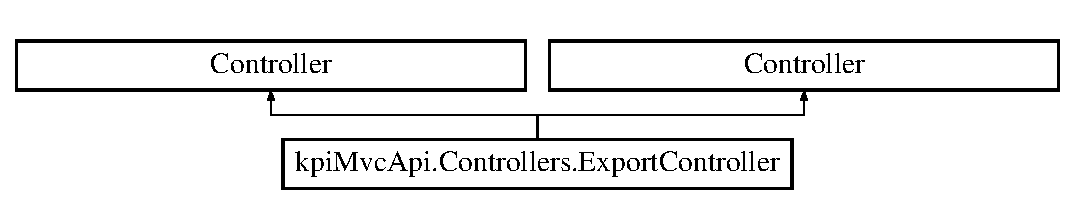
\includegraphics[height=2.000000cm]{classkpi_mvc_api_1_1_controllers_1_1_export_controller}
\end{center}
\end{figure}
\subsection*{Public Member Functions}
\begin{DoxyCompactItemize}
\item 
Action\+Result \hyperlink{classkpi_mvc_api_1_1_controllers_1_1_export_controller_a7f779c9cca92a11fd9c37bfef15c0ad4}{Prod\+Data\+To\+Excel} ()
\begin{DoxyCompactList}\small\item\em Nimmt daten aus dem Production Data Data Transfer Object Recordset Bindet die Daten in eine Gridview Exportiert die Daten in eine Excell.\+xls \end{DoxyCompactList}\item 
Action\+Result \hyperlink{classkpi_mvc_api_1_1_controllers_1_1_export_controller_a5350dfcc0605aeb646490cdedd3374bc}{Kvp\+Data\+To\+Excel} ()
\begin{DoxyCompactList}\small\item\em Nimmt daten aus dem Kvp Data Data Transfer Object Recordset Bindet die Daten in eine Gridview Exportiert die Daten in eine Excell.\+xls \end{DoxyCompactList}\item 
Action\+Result \hyperlink{classkpi_mvc_api_1_1_controllers_1_1_export_controller_a9bfabbfc7273a1c541a8e3bd33ea08e6}{Delivery\+Data\+To\+Excel} ()
\begin{DoxyCompactList}\small\item\em Nimmt daten aus dem Deliovery Data Data Transfer Object Recordset Bindet die Daten in eine Gridview Exportiert die Daten in eine Excell.\+xls \end{DoxyCompactList}\item 
Action\+Result \hyperlink{classkpi_mvc_api_1_1_controllers_1_1_export_controller_a7f779c9cca92a11fd9c37bfef15c0ad4}{Prod\+Data\+To\+Excel} ()
\begin{DoxyCompactList}\small\item\em Nimmt daten aus dem Production Data Data Transfer Object Recordset Bindet die Daten in eine Gridview Exportiert die Daten in eine Excell.\+xls \end{DoxyCompactList}\item 
Action\+Result \hyperlink{classkpi_mvc_api_1_1_controllers_1_1_export_controller_a5350dfcc0605aeb646490cdedd3374bc}{Kvp\+Data\+To\+Excel} ()
\begin{DoxyCompactList}\small\item\em Nimmt daten aus dem Kvp Data Data Transfer Object Recordset Bindet die Daten in eine Gridview Exportiert die Daten in eine Excell.\+xls \end{DoxyCompactList}\item 
Action\+Result \hyperlink{classkpi_mvc_api_1_1_controllers_1_1_export_controller_a5de667891d862c9faa1175625cf563f4}{Delivery\+To\+Excel} ()
\begin{DoxyCompactList}\small\item\em Nimmt daten aus dem Deliovery Data Data Transfer Object Recordset Bindet die Daten in eine Gridview Exportiert die Daten in eine Excell.\+xls \end{DoxyCompactList}\end{DoxyCompactItemize}


\subsection{Detailed Description}
Der Exportkontroller stellt den alle Dienste zur exportierung von Files zur Verfügung. 



\subsection{Member Function Documentation}
\mbox{\Hypertarget{classkpi_mvc_api_1_1_controllers_1_1_export_controller_a9bfabbfc7273a1c541a8e3bd33ea08e6}\label{classkpi_mvc_api_1_1_controllers_1_1_export_controller_a9bfabbfc7273a1c541a8e3bd33ea08e6}} 
\index{kpi\+Mvc\+Api\+::\+Controllers\+::\+Export\+Controller@{kpi\+Mvc\+Api\+::\+Controllers\+::\+Export\+Controller}!Delivery\+Data\+To\+Excel@{Delivery\+Data\+To\+Excel}}
\index{Delivery\+Data\+To\+Excel@{Delivery\+Data\+To\+Excel}!kpi\+Mvc\+Api\+::\+Controllers\+::\+Export\+Controller@{kpi\+Mvc\+Api\+::\+Controllers\+::\+Export\+Controller}}
\subsubsection{\texorpdfstring{Delivery\+Data\+To\+Excel()}{DeliveryDataToExcel()}}
{\footnotesize\ttfamily Action\+Result kpi\+Mvc\+Api.\+Controllers.\+Export\+Controller.\+Delivery\+Data\+To\+Excel (\begin{DoxyParamCaption}{ }\end{DoxyParamCaption})\hspace{0.3cm}{\ttfamily [inline]}}



Nimmt daten aus dem Deliovery Data Data Transfer Object Recordset Bindet die Daten in eine Gridview Exportiert die Daten in eine Excell.\+xls 

\begin{DoxyReturn}{Returns}
View() Excell .xls File 
\end{DoxyReturn}
\mbox{\Hypertarget{classkpi_mvc_api_1_1_controllers_1_1_export_controller_a5de667891d862c9faa1175625cf563f4}\label{classkpi_mvc_api_1_1_controllers_1_1_export_controller_a5de667891d862c9faa1175625cf563f4}} 
\index{kpi\+Mvc\+Api\+::\+Controllers\+::\+Export\+Controller@{kpi\+Mvc\+Api\+::\+Controllers\+::\+Export\+Controller}!Delivery\+To\+Excel@{Delivery\+To\+Excel}}
\index{Delivery\+To\+Excel@{Delivery\+To\+Excel}!kpi\+Mvc\+Api\+::\+Controllers\+::\+Export\+Controller@{kpi\+Mvc\+Api\+::\+Controllers\+::\+Export\+Controller}}
\subsubsection{\texorpdfstring{Delivery\+To\+Excel()}{DeliveryToExcel()}}
{\footnotesize\ttfamily Action\+Result kpi\+Mvc\+Api.\+Controllers.\+Export\+Controller.\+Delivery\+To\+Excel (\begin{DoxyParamCaption}{ }\end{DoxyParamCaption})\hspace{0.3cm}{\ttfamily [inline]}}



Nimmt daten aus dem Deliovery Data Data Transfer Object Recordset Bindet die Daten in eine Gridview Exportiert die Daten in eine Excell.\+xls 

\begin{DoxyReturn}{Returns}
View() Excell .xls File 
\end{DoxyReturn}
\mbox{\Hypertarget{classkpi_mvc_api_1_1_controllers_1_1_export_controller_a5350dfcc0605aeb646490cdedd3374bc}\label{classkpi_mvc_api_1_1_controllers_1_1_export_controller_a5350dfcc0605aeb646490cdedd3374bc}} 
\index{kpi\+Mvc\+Api\+::\+Controllers\+::\+Export\+Controller@{kpi\+Mvc\+Api\+::\+Controllers\+::\+Export\+Controller}!Kvp\+Data\+To\+Excel@{Kvp\+Data\+To\+Excel}}
\index{Kvp\+Data\+To\+Excel@{Kvp\+Data\+To\+Excel}!kpi\+Mvc\+Api\+::\+Controllers\+::\+Export\+Controller@{kpi\+Mvc\+Api\+::\+Controllers\+::\+Export\+Controller}}
\subsubsection{\texorpdfstring{Kvp\+Data\+To\+Excel()}{KvpDataToExcel()}\hspace{0.1cm}{\footnotesize\ttfamily [1/2]}}
{\footnotesize\ttfamily Action\+Result kpi\+Mvc\+Api.\+Controllers.\+Export\+Controller.\+Kvp\+Data\+To\+Excel (\begin{DoxyParamCaption}{ }\end{DoxyParamCaption})\hspace{0.3cm}{\ttfamily [inline]}}



Nimmt daten aus dem Kvp Data Data Transfer Object Recordset Bindet die Daten in eine Gridview Exportiert die Daten in eine Excell.\+xls 

\begin{DoxyReturn}{Returns}
View() Excell .xls File 
\end{DoxyReturn}
\mbox{\Hypertarget{classkpi_mvc_api_1_1_controllers_1_1_export_controller_a5350dfcc0605aeb646490cdedd3374bc}\label{classkpi_mvc_api_1_1_controllers_1_1_export_controller_a5350dfcc0605aeb646490cdedd3374bc}} 
\index{kpi\+Mvc\+Api\+::\+Controllers\+::\+Export\+Controller@{kpi\+Mvc\+Api\+::\+Controllers\+::\+Export\+Controller}!Kvp\+Data\+To\+Excel@{Kvp\+Data\+To\+Excel}}
\index{Kvp\+Data\+To\+Excel@{Kvp\+Data\+To\+Excel}!kpi\+Mvc\+Api\+::\+Controllers\+::\+Export\+Controller@{kpi\+Mvc\+Api\+::\+Controllers\+::\+Export\+Controller}}
\subsubsection{\texorpdfstring{Kvp\+Data\+To\+Excel()}{KvpDataToExcel()}\hspace{0.1cm}{\footnotesize\ttfamily [2/2]}}
{\footnotesize\ttfamily Action\+Result kpi\+Mvc\+Api.\+Controllers.\+Export\+Controller.\+Kvp\+Data\+To\+Excel (\begin{DoxyParamCaption}{ }\end{DoxyParamCaption})\hspace{0.3cm}{\ttfamily [inline]}}



Nimmt daten aus dem Kvp Data Data Transfer Object Recordset Bindet die Daten in eine Gridview Exportiert die Daten in eine Excell.\+xls 

\begin{DoxyReturn}{Returns}
View() Excell .xls File 
\end{DoxyReturn}
\mbox{\Hypertarget{classkpi_mvc_api_1_1_controllers_1_1_export_controller_a7f779c9cca92a11fd9c37bfef15c0ad4}\label{classkpi_mvc_api_1_1_controllers_1_1_export_controller_a7f779c9cca92a11fd9c37bfef15c0ad4}} 
\index{kpi\+Mvc\+Api\+::\+Controllers\+::\+Export\+Controller@{kpi\+Mvc\+Api\+::\+Controllers\+::\+Export\+Controller}!Prod\+Data\+To\+Excel@{Prod\+Data\+To\+Excel}}
\index{Prod\+Data\+To\+Excel@{Prod\+Data\+To\+Excel}!kpi\+Mvc\+Api\+::\+Controllers\+::\+Export\+Controller@{kpi\+Mvc\+Api\+::\+Controllers\+::\+Export\+Controller}}
\subsubsection{\texorpdfstring{Prod\+Data\+To\+Excel()}{ProdDataToExcel()}\hspace{0.1cm}{\footnotesize\ttfamily [1/2]}}
{\footnotesize\ttfamily Action\+Result kpi\+Mvc\+Api.\+Controllers.\+Export\+Controller.\+Prod\+Data\+To\+Excel (\begin{DoxyParamCaption}{ }\end{DoxyParamCaption})\hspace{0.3cm}{\ttfamily [inline]}}



Nimmt daten aus dem Production Data Data Transfer Object Recordset Bindet die Daten in eine Gridview Exportiert die Daten in eine Excell.\+xls 

\begin{DoxyReturn}{Returns}
View() Excell .xls File 
\end{DoxyReturn}
\mbox{\Hypertarget{classkpi_mvc_api_1_1_controllers_1_1_export_controller_a7f779c9cca92a11fd9c37bfef15c0ad4}\label{classkpi_mvc_api_1_1_controllers_1_1_export_controller_a7f779c9cca92a11fd9c37bfef15c0ad4}} 
\index{kpi\+Mvc\+Api\+::\+Controllers\+::\+Export\+Controller@{kpi\+Mvc\+Api\+::\+Controllers\+::\+Export\+Controller}!Prod\+Data\+To\+Excel@{Prod\+Data\+To\+Excel}}
\index{Prod\+Data\+To\+Excel@{Prod\+Data\+To\+Excel}!kpi\+Mvc\+Api\+::\+Controllers\+::\+Export\+Controller@{kpi\+Mvc\+Api\+::\+Controllers\+::\+Export\+Controller}}
\subsubsection{\texorpdfstring{Prod\+Data\+To\+Excel()}{ProdDataToExcel()}\hspace{0.1cm}{\footnotesize\ttfamily [2/2]}}
{\footnotesize\ttfamily Action\+Result kpi\+Mvc\+Api.\+Controllers.\+Export\+Controller.\+Prod\+Data\+To\+Excel (\begin{DoxyParamCaption}{ }\end{DoxyParamCaption})\hspace{0.3cm}{\ttfamily [inline]}}



Nimmt daten aus dem Production Data Data Transfer Object Recordset Bindet die Daten in eine Gridview Exportiert die Daten in eine Excell.\+xls 

\begin{DoxyReturn}{Returns}
View() Excell .xls File 
\end{DoxyReturn}


The documentation for this class was generated from the following file\+:\begin{DoxyCompactItemize}
\item 
C\+:/\+Users/\+Ulysses/\+Documents/01\+\_\+\+Study\+Fhnw/815\+\_\+veri/kpi\+Web\+Mvc/kpi\+Mvc/kpi\+Mvc\+Api/\+Controllers/Export\+Controller.\+cs\end{DoxyCompactItemize}

\hypertarget{classkpi_mvc_api_1_1_global}{}\section{kpi\+Mvc\+Api.\+Global Class Reference}
\label{classkpi_mvc_api_1_1_global}\index{kpi\+Mvc\+Api.\+Global@{kpi\+Mvc\+Api.\+Global}}
Inheritance diagram for kpi\+Mvc\+Api.\+Global\+:\begin{figure}[H]
\begin{center}
\leavevmode
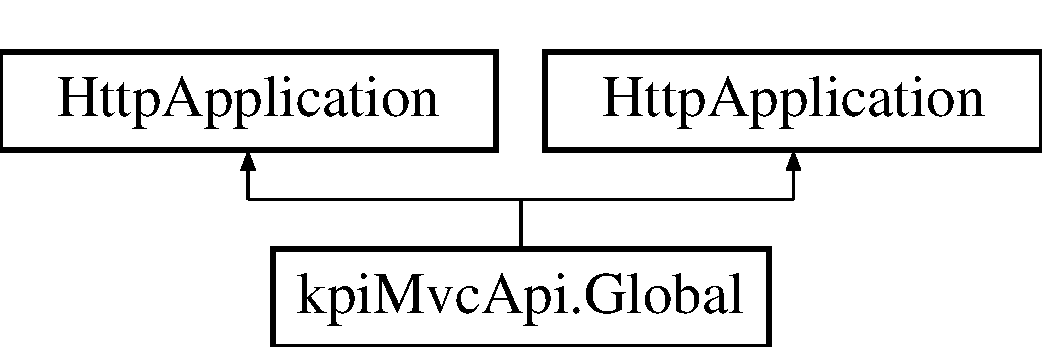
\includegraphics[height=2.000000cm]{classkpi_mvc_api_1_1_global}
\end{center}
\end{figure}


The documentation for this class was generated from the following file\+:\begin{DoxyCompactItemize}
\item 
C\+:/\+Users/\+Ulysses/\+Documents/01\+\_\+\+Study\+Fhnw/815\+\_\+veri/kpi\+Web\+Mvc/kpi\+Mvc/kpi\+Mvc\+Api/Global.\+asax.\+cs\end{DoxyCompactItemize}

\hypertarget{classkpi_mvc_api_1_1_controllers_1_1_home_controller}{}\section{kpi\+Mvc\+Api.\+Controllers.\+Home\+Controller Class Reference}
\label{classkpi_mvc_api_1_1_controllers_1_1_home_controller}\index{kpi\+Mvc\+Api.\+Controllers.\+Home\+Controller@{kpi\+Mvc\+Api.\+Controllers.\+Home\+Controller}}


Webseite Controller Setllt die Views und die Partaialviews bereit  


Inheritance diagram for kpi\+Mvc\+Api.\+Controllers.\+Home\+Controller\+:\begin{figure}[H]
\begin{center}
\leavevmode
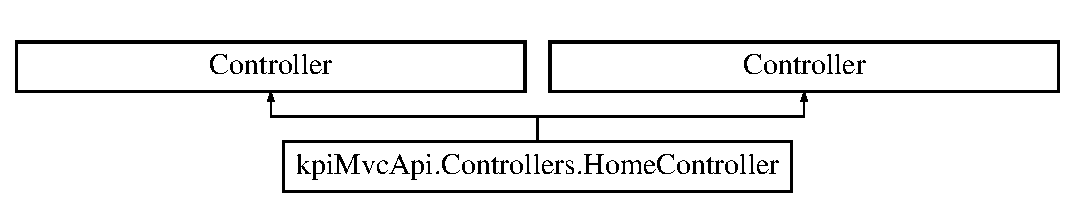
\includegraphics[height=2.000000cm]{classkpi_mvc_api_1_1_controllers_1_1_home_controller}
\end{center}
\end{figure}
\subsection*{Public Member Functions}
\begin{DoxyCompactItemize}
\item 
Action\+Result \hyperlink{classkpi_mvc_api_1_1_controllers_1_1_home_controller_a10e3c3151fdc896f23d1ed374bdcd6cf}{Index} ()
\begin{DoxyCompactList}\small\item\em Test Webseite um Funktionen zu testen \end{DoxyCompactList}\item 
Action\+Result \hyperlink{classkpi_mvc_api_1_1_controllers_1_1_home_controller_a8fe51f06ec9db44e1766f89691af44f6}{Frame} ()
\begin{DoxyCompactList}\small\item\em The Dashboard Frame Returns the Frame\+View withe Menue and Sidebar \end{DoxyCompactList}\item 
Action\+Result \hyperlink{classkpi_mvc_api_1_1_controllers_1_1_home_controller_a71cc0c383f8e44677455f0caf590e0a7}{Home} ()
\begin{DoxyCompactList}\small\item\em The Home View Returns the Home View with Av \end{DoxyCompactList}\item 
Action\+Result \hyperlink{classkpi_mvc_api_1_1_controllers_1_1_home_controller_a52ba84d65a16f3ec9f7c18ef46313b23}{User\+Login} ()
\begin{DoxyCompactList}\small\item\em The User Login View Returns the View to login a User \end{DoxyCompactList}\item 
Action\+Result \hyperlink{classkpi_mvc_api_1_1_controllers_1_1_home_controller_ae5c2fcc4413eda2cab2775cd9819efca}{Production\+Data} (string start\+Date, string stop\+Date)
\begin{DoxyCompactList}\small\item\em The Production Data View Tries to parse the Date Strings to Date\+Time Class The Data is filtered by these Parameters For nonvalid Dates the Standarddate will be loaded \end{DoxyCompactList}\item 
Action\+Result \hyperlink{classkpi_mvc_api_1_1_controllers_1_1_home_controller_aab951608121b90d9424bb58c68bd0b23}{Kvp} (string start\+Date, string stop\+Date)
\begin{DoxyCompactList}\small\item\em The K\+VP View Tries to parse the Date Strings to Date\+Time Class The Data is filtered by these Parameters For nonvalid Dates the Standarddate will be loaded \end{DoxyCompactList}\item 
Action\+Result \hyperlink{classkpi_mvc_api_1_1_controllers_1_1_home_controller_a0fe5ac7be69616c8f56e8938e042cc27}{Delivery} (string start\+Date, string stop\+Date)
\begin{DoxyCompactList}\small\item\em The Delivery View Tries to parse the Date Strings to Date\+Time Class The Data is filtered by these Parameters For nonvalid Dates the Standarddate will be loaded \end{DoxyCompactList}\item 
\mbox{\Hypertarget{classkpi_mvc_api_1_1_controllers_1_1_home_controller_a10e3c3151fdc896f23d1ed374bdcd6cf}\label{classkpi_mvc_api_1_1_controllers_1_1_home_controller_a10e3c3151fdc896f23d1ed374bdcd6cf}} 
Action\+Result {\bfseries Index} ()
\item 
\mbox{\Hypertarget{classkpi_mvc_api_1_1_controllers_1_1_home_controller_a632bd6044f851bdf520c08b6fbf9604e}\label{classkpi_mvc_api_1_1_controllers_1_1_home_controller_a632bd6044f851bdf520c08b6fbf9604e}} 
Action\+Result {\bfseries Export\+To\+Excel} ()
\item 
\mbox{\Hypertarget{classkpi_mvc_api_1_1_controllers_1_1_home_controller_a8fe51f06ec9db44e1766f89691af44f6}\label{classkpi_mvc_api_1_1_controllers_1_1_home_controller_a8fe51f06ec9db44e1766f89691af44f6}} 
Action\+Result {\bfseries Frame} ()
\item 
\mbox{\Hypertarget{classkpi_mvc_api_1_1_controllers_1_1_home_controller_a136db913ab3394130e98d9e9376f2be9}\label{classkpi_mvc_api_1_1_controllers_1_1_home_controller_a136db913ab3394130e98d9e9376f2be9}} 
Action\+Result {\bfseries Home} (string start\+Date, string stop\+Date)
\item 
\mbox{\Hypertarget{classkpi_mvc_api_1_1_controllers_1_1_home_controller_a52ba84d65a16f3ec9f7c18ef46313b23}\label{classkpi_mvc_api_1_1_controllers_1_1_home_controller_a52ba84d65a16f3ec9f7c18ef46313b23}} 
Action\+Result {\bfseries User\+Login} ()
\item 
\mbox{\Hypertarget{classkpi_mvc_api_1_1_controllers_1_1_home_controller_ae5c2fcc4413eda2cab2775cd9819efca}\label{classkpi_mvc_api_1_1_controllers_1_1_home_controller_ae5c2fcc4413eda2cab2775cd9819efca}} 
Action\+Result {\bfseries Production\+Data} (string start\+Date, string stop\+Date)
\item 
\mbox{\Hypertarget{classkpi_mvc_api_1_1_controllers_1_1_home_controller_a2b29fc025ba4bc7cb5be2cf16a4ab4b8}\label{classkpi_mvc_api_1_1_controllers_1_1_home_controller_a2b29fc025ba4bc7cb5be2cf16a4ab4b8}} 
Action\+Result {\bfseries Quality\+Data} ()
\item 
\mbox{\Hypertarget{classkpi_mvc_api_1_1_controllers_1_1_home_controller_aa62132d07d9a778856a532fa6a2112b0}\label{classkpi_mvc_api_1_1_controllers_1_1_home_controller_aa62132d07d9a778856a532fa6a2112b0}} 
Action\+Result {\bfseries Oee} ()
\end{DoxyCompactItemize}


\subsection{Detailed Description}
Webseite Controller Setllt die Views und die Partaialviews bereit 



\subsection{Member Function Documentation}
\mbox{\Hypertarget{classkpi_mvc_api_1_1_controllers_1_1_home_controller_a0fe5ac7be69616c8f56e8938e042cc27}\label{classkpi_mvc_api_1_1_controllers_1_1_home_controller_a0fe5ac7be69616c8f56e8938e042cc27}} 
\index{kpi\+Mvc\+Api\+::\+Controllers\+::\+Home\+Controller@{kpi\+Mvc\+Api\+::\+Controllers\+::\+Home\+Controller}!Delivery@{Delivery}}
\index{Delivery@{Delivery}!kpi\+Mvc\+Api\+::\+Controllers\+::\+Home\+Controller@{kpi\+Mvc\+Api\+::\+Controllers\+::\+Home\+Controller}}
\subsubsection{\texorpdfstring{Delivery()}{Delivery()}}
{\footnotesize\ttfamily Action\+Result kpi\+Mvc\+Api.\+Controllers.\+Home\+Controller.\+Delivery (\begin{DoxyParamCaption}\item[{string}]{start\+Date,  }\item[{string}]{stop\+Date }\end{DoxyParamCaption})\hspace{0.3cm}{\ttfamily [inline]}}



The Delivery View Tries to parse the Date Strings to Date\+Time Class The Data is filtered by these Parameters For nonvalid Dates the Standarddate will be loaded 


\begin{DoxyParams}{Parameters}
{\em start\+Date} & \\
\hline
{\em stop\+Date} & \\
\hline
\end{DoxyParams}
\begin{DoxyReturn}{Returns}
{\ttfamily Partial\+View(\char`\"{}\+\_\+\+Delivery\char`\"{}, model);} The View Containing all selected Delivery Data, shown as a diagram and a Table. Also provide an Excell export function 
\end{DoxyReturn}
\mbox{\Hypertarget{classkpi_mvc_api_1_1_controllers_1_1_home_controller_a8fe51f06ec9db44e1766f89691af44f6}\label{classkpi_mvc_api_1_1_controllers_1_1_home_controller_a8fe51f06ec9db44e1766f89691af44f6}} 
\index{kpi\+Mvc\+Api\+::\+Controllers\+::\+Home\+Controller@{kpi\+Mvc\+Api\+::\+Controllers\+::\+Home\+Controller}!Frame@{Frame}}
\index{Frame@{Frame}!kpi\+Mvc\+Api\+::\+Controllers\+::\+Home\+Controller@{kpi\+Mvc\+Api\+::\+Controllers\+::\+Home\+Controller}}
\subsubsection{\texorpdfstring{Frame()}{Frame()}}
{\footnotesize\ttfamily Action\+Result kpi\+Mvc\+Api.\+Controllers.\+Home\+Controller.\+Frame (\begin{DoxyParamCaption}{ }\end{DoxyParamCaption})\hspace{0.3cm}{\ttfamily [inline]}}



The Dashboard Frame Returns the Frame\+View withe Menue and Sidebar 

\begin{DoxyReturn}{Returns}
Action\+Result Frame\+View
\end{DoxyReturn}
\mbox{\Hypertarget{classkpi_mvc_api_1_1_controllers_1_1_home_controller_a71cc0c383f8e44677455f0caf590e0a7}\label{classkpi_mvc_api_1_1_controllers_1_1_home_controller_a71cc0c383f8e44677455f0caf590e0a7}} 
\index{kpi\+Mvc\+Api\+::\+Controllers\+::\+Home\+Controller@{kpi\+Mvc\+Api\+::\+Controllers\+::\+Home\+Controller}!Home@{Home}}
\index{Home@{Home}!kpi\+Mvc\+Api\+::\+Controllers\+::\+Home\+Controller@{kpi\+Mvc\+Api\+::\+Controllers\+::\+Home\+Controller}}
\subsubsection{\texorpdfstring{Home()}{Home()}}
{\footnotesize\ttfamily Action\+Result kpi\+Mvc\+Api.\+Controllers.\+Home\+Controller.\+Home (\begin{DoxyParamCaption}{ }\end{DoxyParamCaption})\hspace{0.3cm}{\ttfamily [inline]}}



The Home View Returns the Home View with Av 

\begin{DoxyReturn}{Returns}
Action\+Result Home\+View/returns$>$ 
\end{DoxyReturn}
\mbox{\Hypertarget{classkpi_mvc_api_1_1_controllers_1_1_home_controller_a10e3c3151fdc896f23d1ed374bdcd6cf}\label{classkpi_mvc_api_1_1_controllers_1_1_home_controller_a10e3c3151fdc896f23d1ed374bdcd6cf}} 
\index{kpi\+Mvc\+Api\+::\+Controllers\+::\+Home\+Controller@{kpi\+Mvc\+Api\+::\+Controllers\+::\+Home\+Controller}!Index@{Index}}
\index{Index@{Index}!kpi\+Mvc\+Api\+::\+Controllers\+::\+Home\+Controller@{kpi\+Mvc\+Api\+::\+Controllers\+::\+Home\+Controller}}
\subsubsection{\texorpdfstring{Index()}{Index()}}
{\footnotesize\ttfamily Action\+Result kpi\+Mvc\+Api.\+Controllers.\+Home\+Controller.\+Index (\begin{DoxyParamCaption}{ }\end{DoxyParamCaption})\hspace{0.3cm}{\ttfamily [inline]}}



Test Webseite um Funktionen zu testen 

\begin{DoxyReturn}{Returns}
Action\+Result Index\+View
\end{DoxyReturn}
\mbox{\Hypertarget{classkpi_mvc_api_1_1_controllers_1_1_home_controller_aab951608121b90d9424bb58c68bd0b23}\label{classkpi_mvc_api_1_1_controllers_1_1_home_controller_aab951608121b90d9424bb58c68bd0b23}} 
\index{kpi\+Mvc\+Api\+::\+Controllers\+::\+Home\+Controller@{kpi\+Mvc\+Api\+::\+Controllers\+::\+Home\+Controller}!Kvp@{Kvp}}
\index{Kvp@{Kvp}!kpi\+Mvc\+Api\+::\+Controllers\+::\+Home\+Controller@{kpi\+Mvc\+Api\+::\+Controllers\+::\+Home\+Controller}}
\subsubsection{\texorpdfstring{Kvp()}{Kvp()}}
{\footnotesize\ttfamily Action\+Result kpi\+Mvc\+Api.\+Controllers.\+Home\+Controller.\+Kvp (\begin{DoxyParamCaption}\item[{string}]{start\+Date,  }\item[{string}]{stop\+Date }\end{DoxyParamCaption})\hspace{0.3cm}{\ttfamily [inline]}}



The K\+VP View Tries to parse the Date Strings to Date\+Time Class The Data is filtered by these Parameters For nonvalid Dates the Standarddate will be loaded 


\begin{DoxyParams}{Parameters}
{\em start\+Date} & \\
\hline
{\em stop\+Date} & \\
\hline
\end{DoxyParams}
\begin{DoxyReturn}{Returns}
{\ttfamily Partial\+View(\char`\"{}\+\_\+\+Kvp\char`\"{}, model);} The View Containing all selected K\+VP Data, shown as a diagram and a List. Also provide an Excell export function 
\end{DoxyReturn}
\mbox{\Hypertarget{classkpi_mvc_api_1_1_controllers_1_1_home_controller_ae5c2fcc4413eda2cab2775cd9819efca}\label{classkpi_mvc_api_1_1_controllers_1_1_home_controller_ae5c2fcc4413eda2cab2775cd9819efca}} 
\index{kpi\+Mvc\+Api\+::\+Controllers\+::\+Home\+Controller@{kpi\+Mvc\+Api\+::\+Controllers\+::\+Home\+Controller}!Production\+Data@{Production\+Data}}
\index{Production\+Data@{Production\+Data}!kpi\+Mvc\+Api\+::\+Controllers\+::\+Home\+Controller@{kpi\+Mvc\+Api\+::\+Controllers\+::\+Home\+Controller}}
\subsubsection{\texorpdfstring{Production\+Data()}{ProductionData()}}
{\footnotesize\ttfamily Action\+Result kpi\+Mvc\+Api.\+Controllers.\+Home\+Controller.\+Production\+Data (\begin{DoxyParamCaption}\item[{string}]{start\+Date,  }\item[{string}]{stop\+Date }\end{DoxyParamCaption})\hspace{0.3cm}{\ttfamily [inline]}}



The Production Data View Tries to parse the Date Strings to Date\+Time Class The Data is filtered by these Parameters For nonvalid Dates the Standarddate will be loaded 


\begin{DoxyParams}{Parameters}
{\em start\+Date} & The Date the Dataset starts\\
\hline
{\em stop\+Date} & The Date the Dataset stops \\
\hline
\end{DoxyParams}
\begin{DoxyReturn}{Returns}
{\ttfamily Action\+Result Partial\+View(\char`\"{}\+\_\+\+Production\+Data\char`\"{}, model);} The View containing all selected Production Date, shown as a diagram and a table. Also provide an Excell export function 
\end{DoxyReturn}
\mbox{\Hypertarget{classkpi_mvc_api_1_1_controllers_1_1_home_controller_a52ba84d65a16f3ec9f7c18ef46313b23}\label{classkpi_mvc_api_1_1_controllers_1_1_home_controller_a52ba84d65a16f3ec9f7c18ef46313b23}} 
\index{kpi\+Mvc\+Api\+::\+Controllers\+::\+Home\+Controller@{kpi\+Mvc\+Api\+::\+Controllers\+::\+Home\+Controller}!User\+Login@{User\+Login}}
\index{User\+Login@{User\+Login}!kpi\+Mvc\+Api\+::\+Controllers\+::\+Home\+Controller@{kpi\+Mvc\+Api\+::\+Controllers\+::\+Home\+Controller}}
\subsubsection{\texorpdfstring{User\+Login()}{UserLogin()}}
{\footnotesize\ttfamily Action\+Result kpi\+Mvc\+Api.\+Controllers.\+Home\+Controller.\+User\+Login (\begin{DoxyParamCaption}{ }\end{DoxyParamCaption})\hspace{0.3cm}{\ttfamily [inline]}}



The User Login View Returns the View to login a User 

\begin{DoxyReturn}{Returns}
Action\+Result User\+Login\+View
\end{DoxyReturn}


The documentation for this class was generated from the following file\+:\begin{DoxyCompactItemize}
\item 
C\+:/\+Users/\+Ulysses/\+Documents/01\+\_\+\+Study\+Fhnw/815\+\_\+veri/kpi\+Web\+Mvc/kpi\+Mvc/kpi\+Mvc\+Api/\+Controllers/Home\+Controller.\+cs\end{DoxyCompactItemize}

\hypertarget{classkpi_mvc_api_1_1_controllers_1_1_kpidata_controller}{}\section{kpi\+Mvc\+Api.\+Controllers.\+Kpidata\+Controller Class Reference}
\label{classkpi_mvc_api_1_1_controllers_1_1_kpidata_controller}\index{kpi\+Mvc\+Api.\+Controllers.\+Kpidata\+Controller@{kpi\+Mvc\+Api.\+Controllers.\+Kpidata\+Controller}}
Inheritance diagram for kpi\+Mvc\+Api.\+Controllers.\+Kpidata\+Controller\+:\begin{figure}[H]
\begin{center}
\leavevmode
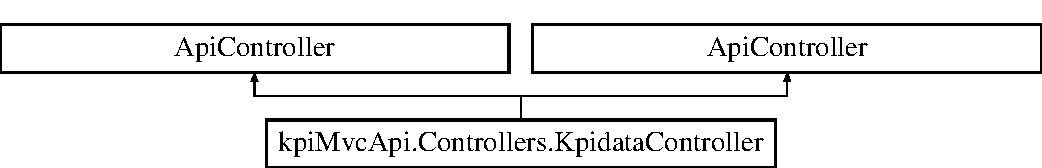
\includegraphics[height=2.000000cm]{classkpi_mvc_api_1_1_controllers_1_1_kpidata_controller}
\end{center}
\end{figure}
\subsection*{Public Member Functions}
\begin{DoxyCompactItemize}
\item 
\mbox{\Hypertarget{classkpi_mvc_api_1_1_controllers_1_1_kpidata_controller_a0ab15672f7d3b5a077a8c4b0612feab8}\label{classkpi_mvc_api_1_1_controllers_1_1_kpidata_controller_a0ab15672f7d3b5a077a8c4b0612feab8}} 
List$<$ \hyperlink{classkpi_mvc_api_1_1_data_transfer_objects_1_1_production_data_dto}{Production\+Data\+Dto} $>$ {\bfseries get\+Production\+Data} ()
\item 
\mbox{\Hypertarget{classkpi_mvc_api_1_1_controllers_1_1_kpidata_controller_a7f6c6c359f37a9b9a83d481b5c26a037}\label{classkpi_mvc_api_1_1_controllers_1_1_kpidata_controller_a7f6c6c359f37a9b9a83d481b5c26a037}} 
Http\+Response\+Message {\bfseries set\+Production\+Data} (List$<$ \hyperlink{classkpi_mvc_api_1_1_data_transfer_objects_1_1_production_data_dto}{Production\+Data\+Dto} $>$ prod\+Data\+List)
\item 
\mbox{\Hypertarget{classkpi_mvc_api_1_1_controllers_1_1_kpidata_controller_a82f308e9ae4809dfdca3ce685af05774}\label{classkpi_mvc_api_1_1_controllers_1_1_kpidata_controller_a82f308e9ae4809dfdca3ce685af05774}} 
Http\+Response\+Message {\bfseries update\+Production\+Data} (List$<$ \hyperlink{classkpi_mvc_api_1_1_data_transfer_objects_1_1_production_data_dto}{Production\+Data\+Dto} $>$ prod\+Data\+List)
\item 
\mbox{\Hypertarget{classkpi_mvc_api_1_1_controllers_1_1_kpidata_controller_af1c1e99336a8408bbe4b637cfaaddc4b}\label{classkpi_mvc_api_1_1_controllers_1_1_kpidata_controller_af1c1e99336a8408bbe4b637cfaaddc4b}} 
Http\+Response\+Message {\bfseries delete\+Production\+Data} (List$<$ \hyperlink{classkpi_mvc_api_1_1_data_transfer_objects_1_1_production_data_dto}{Production\+Data\+Dto} $>$ prod\+Data\+List)
\item 
\mbox{\Hypertarget{classkpi_mvc_api_1_1_controllers_1_1_kpidata_controller_ae5b9cebd2043650b2fd60caa72e49da7}\label{classkpi_mvc_api_1_1_controllers_1_1_kpidata_controller_ae5b9cebd2043650b2fd60caa72e49da7}} 
List$<$ \hyperlink{classkpi_mvc_api_1_1_data_transfer_objects_1_1_kvp_data_dto}{Kvp\+Data\+Dto} $>$ {\bfseries get\+Kvp\+Data} ()
\item 
\mbox{\Hypertarget{classkpi_mvc_api_1_1_controllers_1_1_kpidata_controller_aaed21921287f9a780cc3ff7e1042dc2a}\label{classkpi_mvc_api_1_1_controllers_1_1_kpidata_controller_aaed21921287f9a780cc3ff7e1042dc2a}} 
Http\+Response\+Message {\bfseries set\+Kvp\+Data} (List$<$ \hyperlink{classkpi_mvc_api_1_1_data_transfer_objects_1_1_kvp_data_dto}{Kvp\+Data\+Dto} $>$ kvp\+Data\+List)
\item 
\mbox{\Hypertarget{classkpi_mvc_api_1_1_controllers_1_1_kpidata_controller_ac165b3dedfa1744a41af6a1acc07a657}\label{classkpi_mvc_api_1_1_controllers_1_1_kpidata_controller_ac165b3dedfa1744a41af6a1acc07a657}} 
Http\+Response\+Message {\bfseries update\+Kvp\+Data} (List$<$ \hyperlink{classkpi_mvc_api_1_1_data_transfer_objects_1_1_kvp_data_dto}{Kvp\+Data\+Dto} $>$ kvp\+Data\+List)
\item 
\mbox{\Hypertarget{classkpi_mvc_api_1_1_controllers_1_1_kpidata_controller_a42bfeef2bf903c70d9d8452367ed6dd0}\label{classkpi_mvc_api_1_1_controllers_1_1_kpidata_controller_a42bfeef2bf903c70d9d8452367ed6dd0}} 
Http\+Response\+Message {\bfseries delete\+Kvp\+Data} (List$<$ \hyperlink{classkpi_mvc_api_1_1_data_transfer_objects_1_1_kvp_data_dto}{Kvp\+Data\+Dto} $>$ kvp\+Id)
\item 
\mbox{\Hypertarget{classkpi_mvc_api_1_1_controllers_1_1_kpidata_controller_a731d149b7c58ba7de0a45c2eb3110fe1}\label{classkpi_mvc_api_1_1_controllers_1_1_kpidata_controller_a731d149b7c58ba7de0a45c2eb3110fe1}} 
List$<$ \hyperlink{classkpi_mvc_api_1_1_data_transfer_objects_1_1_delivery_data_dto}{Delivery\+Data\+Dto} $>$ {\bfseries get\+Delivery\+Data} ()
\item 
\mbox{\Hypertarget{classkpi_mvc_api_1_1_controllers_1_1_kpidata_controller_ae0c16d6b3d009224eae6ea5a2b20aabd}\label{classkpi_mvc_api_1_1_controllers_1_1_kpidata_controller_ae0c16d6b3d009224eae6ea5a2b20aabd}} 
Http\+Response\+Message {\bfseries set\+Delivery\+Data} (List$<$ \hyperlink{classkpi_mvc_api_1_1_data_transfer_objects_1_1_delivery_data_dto}{Delivery\+Data\+Dto} $>$ delivery\+Data\+List)
\item 
\mbox{\Hypertarget{classkpi_mvc_api_1_1_controllers_1_1_kpidata_controller_a893e7ff73b6dbd31afa5e1aa73e5abae}\label{classkpi_mvc_api_1_1_controllers_1_1_kpidata_controller_a893e7ff73b6dbd31afa5e1aa73e5abae}} 
Http\+Response\+Message {\bfseries update\+Delivery\+Data} (List$<$ \hyperlink{classkpi_mvc_api_1_1_data_transfer_objects_1_1_delivery_data_dto}{Delivery\+Data\+Dto} $>$ delivery\+Data\+List)
\item 
\mbox{\Hypertarget{classkpi_mvc_api_1_1_controllers_1_1_kpidata_controller_a2494970082b1b00fd50353e4aa840188}\label{classkpi_mvc_api_1_1_controllers_1_1_kpidata_controller_a2494970082b1b00fd50353e4aa840188}} 
Http\+Response\+Message {\bfseries delete\+Delivery\+Data} (List$<$ \hyperlink{classkpi_mvc_api_1_1_data_transfer_objects_1_1_delivery_data_dto}{Delivery\+Data\+Dto} $>$ delivery\+Data\+List)
\item 
\mbox{\Hypertarget{classkpi_mvc_api_1_1_controllers_1_1_kpidata_controller_a0ab15672f7d3b5a077a8c4b0612feab8}\label{classkpi_mvc_api_1_1_controllers_1_1_kpidata_controller_a0ab15672f7d3b5a077a8c4b0612feab8}} 
List$<$ \hyperlink{classkpi_mvc_api_1_1_data_transfer_objects_1_1_production_data_dto}{Production\+Data\+Dto} $>$ {\bfseries get\+Production\+Data} ()
\item 
\mbox{\Hypertarget{classkpi_mvc_api_1_1_controllers_1_1_kpidata_controller_a7f6c6c359f37a9b9a83d481b5c26a037}\label{classkpi_mvc_api_1_1_controllers_1_1_kpidata_controller_a7f6c6c359f37a9b9a83d481b5c26a037}} 
Http\+Response\+Message {\bfseries set\+Production\+Data} (List$<$ \hyperlink{classkpi_mvc_api_1_1_data_transfer_objects_1_1_production_data_dto}{Production\+Data\+Dto} $>$ prod\+Data\+List)
\end{DoxyCompactItemize}


The documentation for this class was generated from the following file\+:\begin{DoxyCompactItemize}
\item 
C\+:/\+Users/\+Ulysses/\+Documents/01\+\_\+\+Study\+Fhnw/815\+\_\+veri/kpi\+Web\+Mvc/kpi\+Mvc/kpi\+Mvc\+Api/\+Controllers/Kpidata\+Controller.\+cs\end{DoxyCompactItemize}

\hypertarget{classkpi_mvc_api_1_1_models_1_1kpidb_entities1}{}\section{kpi\+Mvc\+Api.\+Models.\+kpidb\+Entities1 Class Reference}
\label{classkpi_mvc_api_1_1_models_1_1kpidb_entities1}\index{kpi\+Mvc\+Api.\+Models.\+kpidb\+Entities1@{kpi\+Mvc\+Api.\+Models.\+kpidb\+Entities1}}
Inheritance diagram for kpi\+Mvc\+Api.\+Models.\+kpidb\+Entities1\+:\begin{figure}[H]
\begin{center}
\leavevmode
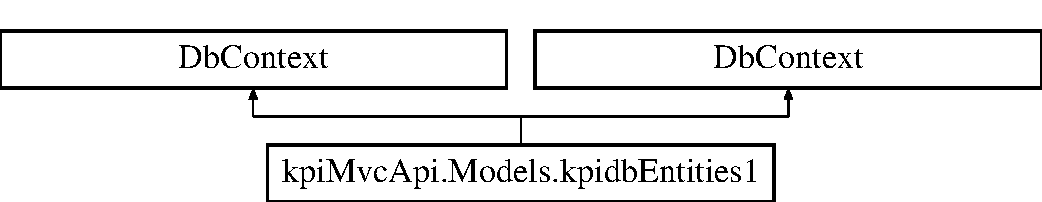
\includegraphics[height=2.000000cm]{classkpi_mvc_api_1_1_models_1_1kpidb_entities1}
\end{center}
\end{figure}
\subsection*{Protected Member Functions}
\begin{DoxyCompactItemize}
\item 
\mbox{\Hypertarget{classkpi_mvc_api_1_1_models_1_1kpidb_entities1_a08bd4559ef70af9b3d494f820e87f8f2}\label{classkpi_mvc_api_1_1_models_1_1kpidb_entities1_a08bd4559ef70af9b3d494f820e87f8f2}} 
override void {\bfseries On\+Model\+Creating} (Db\+Model\+Builder model\+Builder)
\item 
\mbox{\Hypertarget{classkpi_mvc_api_1_1_models_1_1kpidb_entities1_a08bd4559ef70af9b3d494f820e87f8f2}\label{classkpi_mvc_api_1_1_models_1_1kpidb_entities1_a08bd4559ef70af9b3d494f820e87f8f2}} 
override void {\bfseries On\+Model\+Creating} (Db\+Model\+Builder model\+Builder)
\end{DoxyCompactItemize}
\subsection*{Properties}
\begin{DoxyCompactItemize}
\item 
\mbox{\Hypertarget{classkpi_mvc_api_1_1_models_1_1kpidb_entities1_ab0c3f6b95970dff141aa1008839933b2}\label{classkpi_mvc_api_1_1_models_1_1kpidb_entities1_ab0c3f6b95970dff141aa1008839933b2}} 
virtual Db\+Set$<$ \hyperlink{classkpi_mvc_api_1_1_models_1_1e_pcb_class}{e\+Pcb\+Class} $>$ {\bfseries e\+Pcb\+Classes}\hspace{0.3cm}{\ttfamily  \mbox{[}get, set\mbox{]}}
\item 
\mbox{\Hypertarget{classkpi_mvc_api_1_1_models_1_1kpidb_entities1_a424c2ad2fee23f64f20da31a1ae03af9}\label{classkpi_mvc_api_1_1_models_1_1kpidb_entities1_a424c2ad2fee23f64f20da31a1ae03af9}} 
virtual Db\+Set$<$ \hyperlink{classkpi_mvc_api_1_1_models_1_1e_pcb_daily}{e\+Pcb\+Daily} $>$ {\bfseries e\+Pcb\+Dailies}\hspace{0.3cm}{\ttfamily  \mbox{[}get, set\mbox{]}}
\item 
\mbox{\Hypertarget{classkpi_mvc_api_1_1_models_1_1kpidb_entities1_a5c930c131c6a8883a5c5c09e256ac766}\label{classkpi_mvc_api_1_1_models_1_1kpidb_entities1_a5c930c131c6a8883a5c5c09e256ac766}} 
virtual Db\+Set$<$ \hyperlink{classkpi_mvc_api_1_1_models_1_1e_pcb_generation}{e\+Pcb\+Generation} $>$ {\bfseries e\+Pcb\+Generations}\hspace{0.3cm}{\ttfamily  \mbox{[}get, set\mbox{]}}
\item 
\mbox{\Hypertarget{classkpi_mvc_api_1_1_models_1_1kpidb_entities1_a82b2cd1323471107f10b2d875b323569}\label{classkpi_mvc_api_1_1_models_1_1kpidb_entities1_a82b2cd1323471107f10b2d875b323569}} 
virtual Db\+Set$<$ \hyperlink{classkpi_mvc_api_1_1_models_1_1e_kvp}{e\+Kvp} $>$ {\bfseries e\+Kvps}\hspace{0.3cm}{\ttfamily  \mbox{[}get, set\mbox{]}}
\item 
\mbox{\Hypertarget{classkpi_mvc_api_1_1_models_1_1kpidb_entities1_ad552b1e8bf78b0b9abe5698698b0c2fc}\label{classkpi_mvc_api_1_1_models_1_1kpidb_entities1_ad552b1e8bf78b0b9abe5698698b0c2fc}} 
virtual Db\+Set$<$ \hyperlink{classkpi_mvc_api_1_1_models_1_1e_kvp_class}{e\+Kvp\+Class} $>$ {\bfseries e\+Kvp\+Classes}\hspace{0.3cm}{\ttfamily  \mbox{[}get, set\mbox{]}}
\item 
\mbox{\Hypertarget{classkpi_mvc_api_1_1_models_1_1kpidb_entities1_a65dc7b5853f62b29d67129015019bdd7}\label{classkpi_mvc_api_1_1_models_1_1kpidb_entities1_a65dc7b5853f62b29d67129015019bdd7}} 
virtual Db\+Set$<$ \hyperlink{classkpi_mvc_api_1_1_models_1_1e_kvp_state}{e\+Kvp\+State} $>$ {\bfseries e\+Kvp\+States}\hspace{0.3cm}{\ttfamily  \mbox{[}get, set\mbox{]}}
\item 
\mbox{\Hypertarget{classkpi_mvc_api_1_1_models_1_1kpidb_entities1_a4dc3f1977f03dcb917bb6b2e22fb069b}\label{classkpi_mvc_api_1_1_models_1_1kpidb_entities1_a4dc3f1977f03dcb917bb6b2e22fb069b}} 
virtual Db\+Set$<$ \hyperlink{classkpi_mvc_api_1_1_models_1_1e_country}{e\+Country} $>$ {\bfseries e\+Countries}\hspace{0.3cm}{\ttfamily  \mbox{[}get, set\mbox{]}}
\item 
\mbox{\Hypertarget{classkpi_mvc_api_1_1_models_1_1kpidb_entities1_aa8003f98fa22ca806d4a4d989e9b8cbb}\label{classkpi_mvc_api_1_1_models_1_1kpidb_entities1_aa8003f98fa22ca806d4a4d989e9b8cbb}} 
virtual Db\+Set$<$ \hyperlink{classkpi_mvc_api_1_1_models_1_1e_delivery}{e\+Delivery} $>$ {\bfseries e\+Deliveries}\hspace{0.3cm}{\ttfamily  \mbox{[}get, set\mbox{]}}
\end{DoxyCompactItemize}


The documentation for this class was generated from the following file\+:\begin{DoxyCompactItemize}
\item 
C\+:/\+Users/\+Ulysses/\+Documents/01\+\_\+\+Study\+Fhnw/815\+\_\+veri/kpi\+Web\+Mvc/kpi\+Mvc/kpi\+Mvc\+Api/\+Models/azure\+Kpi\+Data.\+Context.\+cs\end{DoxyCompactItemize}

\hypertarget{classkpi_mvc_api_1_1_data_transfer_objects_1_1_kvp_data_dto}{}\section{kpi\+Mvc\+Api.\+Data\+Transfer\+Objects.\+Kvp\+Data\+Dto Class Reference}
\label{classkpi_mvc_api_1_1_data_transfer_objects_1_1_kvp_data_dto}\index{kpi\+Mvc\+Api.\+Data\+Transfer\+Objects.\+Kvp\+Data\+Dto@{kpi\+Mvc\+Api.\+Data\+Transfer\+Objects.\+Kvp\+Data\+Dto}}
\subsection*{Properties}
\begin{DoxyCompactItemize}
\item 
\mbox{\Hypertarget{classkpi_mvc_api_1_1_data_transfer_objects_1_1_kvp_data_dto_a1103688249e2695ac1d5016f7697507e}\label{classkpi_mvc_api_1_1_data_transfer_objects_1_1_kvp_data_dto_a1103688249e2695ac1d5016f7697507e}} 
int {\bfseries Kvp\+Id}\hspace{0.3cm}{\ttfamily  \mbox{[}get, set\mbox{]}}
\item 
\mbox{\Hypertarget{classkpi_mvc_api_1_1_data_transfer_objects_1_1_kvp_data_dto_a67f262168594839cef344d8977cbea79}\label{classkpi_mvc_api_1_1_data_transfer_objects_1_1_kvp_data_dto_a67f262168594839cef344d8977cbea79}} 
string {\bfseries Kvp\+Name}\hspace{0.3cm}{\ttfamily  \mbox{[}get, set\mbox{]}}
\item 
\mbox{\Hypertarget{classkpi_mvc_api_1_1_data_transfer_objects_1_1_kvp_data_dto_a2cb5cacd66158e32ce2401899e72637c}\label{classkpi_mvc_api_1_1_data_transfer_objects_1_1_kvp_data_dto_a2cb5cacd66158e32ce2401899e72637c}} 
Date\+Time {\bfseries Kvp\+Date}\hspace{0.3cm}{\ttfamily  \mbox{[}get, set\mbox{]}}
\item 
\mbox{\Hypertarget{classkpi_mvc_api_1_1_data_transfer_objects_1_1_kvp_data_dto_a2587ba59c5331b2c91c96be4d3131c23}\label{classkpi_mvc_api_1_1_data_transfer_objects_1_1_kvp_data_dto_a2587ba59c5331b2c91c96be4d3131c23}} 
int {\bfseries Kvp\+Class\+Id}\hspace{0.3cm}{\ttfamily  \mbox{[}get, set\mbox{]}}
\item 
\mbox{\Hypertarget{classkpi_mvc_api_1_1_data_transfer_objects_1_1_kvp_data_dto_a725acba0533573b18eade6008d609490}\label{classkpi_mvc_api_1_1_data_transfer_objects_1_1_kvp_data_dto_a725acba0533573b18eade6008d609490}} 
int {\bfseries Kvp\+State\+Id}\hspace{0.3cm}{\ttfamily  \mbox{[}get, set\mbox{]}}
\item 
\mbox{\Hypertarget{classkpi_mvc_api_1_1_data_transfer_objects_1_1_kvp_data_dto_a51355ea3d90f7f8df5296dabf8a53fef}\label{classkpi_mvc_api_1_1_data_transfer_objects_1_1_kvp_data_dto_a51355ea3d90f7f8df5296dabf8a53fef}} 
string {\bfseries Kvp\+State\+Name}\hspace{0.3cm}{\ttfamily  \mbox{[}get, set\mbox{]}}
\item 
\mbox{\Hypertarget{classkpi_mvc_api_1_1_data_transfer_objects_1_1_kvp_data_dto_af58459f2fe09d39cb1caf862456a944f}\label{classkpi_mvc_api_1_1_data_transfer_objects_1_1_kvp_data_dto_af58459f2fe09d39cb1caf862456a944f}} 
string {\bfseries Kvp\+Class\+Name}\hspace{0.3cm}{\ttfamily  \mbox{[}get, set\mbox{]}}
\end{DoxyCompactItemize}


The documentation for this class was generated from the following file\+:\begin{DoxyCompactItemize}
\item 
C\+:/\+Users/i00202128/\+Source/\+Repos/kpi\+Web\+Mvc/kpi\+Mvc/kpi\+Mvc\+Api/\+Data\+Transfer\+Objects/Kvp\+Data\+Dto.\+cs\end{DoxyCompactItemize}

\hypertarget{classkpi_mvc_api_1_1_data_transfer_objects_1_1_kvp_data_dto_rs}{}\section{kpi\+Mvc\+Api.\+Data\+Transfer\+Objects.\+Kvp\+Data\+Dto\+Rs Class Reference}
\label{classkpi_mvc_api_1_1_data_transfer_objects_1_1_kvp_data_dto_rs}\index{kpi\+Mvc\+Api.\+Data\+Transfer\+Objects.\+Kvp\+Data\+Dto\+Rs@{kpi\+Mvc\+Api.\+Data\+Transfer\+Objects.\+Kvp\+Data\+Dto\+Rs}}
\subsection*{Public Types}
\begin{DoxyCompactItemize}
\item 
\mbox{\Hypertarget{classkpi_mvc_api_1_1_data_transfer_objects_1_1_kvp_data_dto_rs_aec5ef29d115053aa1f78d15adc7e1373}\label{classkpi_mvc_api_1_1_data_transfer_objects_1_1_kvp_data_dto_rs_aec5ef29d115053aa1f78d15adc7e1373}} 
enum {\bfseries dataset} \{ {\bfseries Datalabels} = 0, 
{\bfseries dataset1}, 
{\bfseries Datalabels} = 0, 
{\bfseries dataset1}
 \}
\item 
\mbox{\Hypertarget{classkpi_mvc_api_1_1_data_transfer_objects_1_1_kvp_data_dto_rs_a829c595d537885ae923de884be501246}\label{classkpi_mvc_api_1_1_data_transfer_objects_1_1_kvp_data_dto_rs_a829c595d537885ae923de884be501246}} 
enum {\bfseries charttype} \{ {\bfseries Kvp\+Month\+Chart} =0, 
{\bfseries Kvp\+Month\+Chart} =0
 \}
\item 
\mbox{\Hypertarget{classkpi_mvc_api_1_1_data_transfer_objects_1_1_kvp_data_dto_rs_aec5ef29d115053aa1f78d15adc7e1373}\label{classkpi_mvc_api_1_1_data_transfer_objects_1_1_kvp_data_dto_rs_aec5ef29d115053aa1f78d15adc7e1373}} 
enum {\bfseries dataset} \{ {\bfseries Datalabels} = 0, 
{\bfseries dataset1}, 
{\bfseries Datalabels} = 0, 
{\bfseries dataset1}
 \}
\item 
\mbox{\Hypertarget{classkpi_mvc_api_1_1_data_transfer_objects_1_1_kvp_data_dto_rs_a829c595d537885ae923de884be501246}\label{classkpi_mvc_api_1_1_data_transfer_objects_1_1_kvp_data_dto_rs_a829c595d537885ae923de884be501246}} 
enum {\bfseries charttype} \{ {\bfseries Kvp\+Month\+Chart} =0, 
{\bfseries Kvp\+Month\+Chart} =0
 \}
\end{DoxyCompactItemize}
\subsection*{Public Member Functions}
\begin{DoxyCompactItemize}
\item 
\mbox{\Hypertarget{classkpi_mvc_api_1_1_data_transfer_objects_1_1_kvp_data_dto_rs_a4d9df8d729c0009c23968a0250d45dcc}\label{classkpi_mvc_api_1_1_data_transfer_objects_1_1_kvp_data_dto_rs_a4d9df8d729c0009c23968a0250d45dcc}} 
{\bfseries Kvp\+Data\+Dto\+Rs} (Date\+Time startdate, Date\+Time stopdate)
\item 
\mbox{\Hypertarget{classkpi_mvc_api_1_1_data_transfer_objects_1_1_kvp_data_dto_rs_a562207c4315e1f552734257d994cc2d5}\label{classkpi_mvc_api_1_1_data_transfer_objects_1_1_kvp_data_dto_rs_a562207c4315e1f552734257d994cc2d5}} 
void {\bfseries load\+Data} ()
\item 
\mbox{\Hypertarget{classkpi_mvc_api_1_1_data_transfer_objects_1_1_kvp_data_dto_rs_afbda5e8db6a5f8b25125d2a6b6dcf7e1}\label{classkpi_mvc_api_1_1_data_transfer_objects_1_1_kvp_data_dto_rs_afbda5e8db6a5f8b25125d2a6b6dcf7e1}} 
void {\bfseries load\+Data} (Date\+Time startdate, Date\+Time stopdate)
\item 
\mbox{\Hypertarget{classkpi_mvc_api_1_1_data_transfer_objects_1_1_kvp_data_dto_rs_a895f4b97fb8c74c1a853145c03f5d393}\label{classkpi_mvc_api_1_1_data_transfer_objects_1_1_kvp_data_dto_rs_a895f4b97fb8c74c1a853145c03f5d393}} 
List$<$ \hyperlink{classkpi_mvc_api_1_1_data_transfer_objects_1_1_kvp_data_dto}{Kvp\+Data\+Dto} $>$ {\bfseries get\+Data} ()
\item 
\mbox{\Hypertarget{classkpi_mvc_api_1_1_data_transfer_objects_1_1_kvp_data_dto_rs_ac6493e99d1c2fc236a25b61bc51014f9}\label{classkpi_mvc_api_1_1_data_transfer_objects_1_1_kvp_data_dto_rs_ac6493e99d1c2fc236a25b61bc51014f9}} 
List$<$ \hyperlink{classkpi_mvc_api_1_1_data_transfer_objects_1_1_kvp_data_dto}{Kvp\+Data\+Dto} $>$ {\bfseries get\+Data} (Date\+Time startdate, Date\+Time stopdate)
\item 
\mbox{\Hypertarget{classkpi_mvc_api_1_1_data_transfer_objects_1_1_kvp_data_dto_rs_aab05e9ab80b2e766a6744a200e4d8e91}\label{classkpi_mvc_api_1_1_data_transfer_objects_1_1_kvp_data_dto_rs_aab05e9ab80b2e766a6744a200e4d8e91}} 
bool {\bfseries set\+Data} (List$<$ \hyperlink{classkpi_mvc_api_1_1_data_transfer_objects_1_1_kvp_data_dto}{Kvp\+Data\+Dto} $>$ kvpdto)
\item 
\mbox{\Hypertarget{classkpi_mvc_api_1_1_data_transfer_objects_1_1_kvp_data_dto_rs_a9aa97ab6777b36a033c3662e86239e81}\label{classkpi_mvc_api_1_1_data_transfer_objects_1_1_kvp_data_dto_rs_a9aa97ab6777b36a033c3662e86239e81}} 
string {\bfseries get\+Dataset} (charttype charttype, dataset datset, string group\+Mode)
\item 
\mbox{\Hypertarget{classkpi_mvc_api_1_1_data_transfer_objects_1_1_kvp_data_dto_rs_ac1bd4b0312a7a0a07b8848d9cdf739da}\label{classkpi_mvc_api_1_1_data_transfer_objects_1_1_kvp_data_dto_rs_ac1bd4b0312a7a0a07b8848d9cdf739da}} 
List$<$ \hyperlink{classkpi_mvc_api_1_1_data_transfer_objects_1_1_kvp_data_dto}{Kvp\+Data\+Dto} $>$ {\bfseries get\+Kvp\+List} ()
\item 
\mbox{\Hypertarget{classkpi_mvc_api_1_1_data_transfer_objects_1_1_kvp_data_dto_rs_a29e122aca7de38b447056485ad8b4afa}\label{classkpi_mvc_api_1_1_data_transfer_objects_1_1_kvp_data_dto_rs_a29e122aca7de38b447056485ad8b4afa}} 
string {\bfseries get\+Dataset\+Label} ()
\item 
\mbox{\Hypertarget{classkpi_mvc_api_1_1_data_transfer_objects_1_1_kvp_data_dto_rs_ac08415561811e16a01e4fa425709905b}\label{classkpi_mvc_api_1_1_data_transfer_objects_1_1_kvp_data_dto_rs_ac08415561811e16a01e4fa425709905b}} 
string {\bfseries get\+Datset\+Backround\+Color} ()
\item 
\mbox{\Hypertarget{classkpi_mvc_api_1_1_data_transfer_objects_1_1_kvp_data_dto_rs_ac1a9b5ca7012ddd12549e157929f23e7}\label{classkpi_mvc_api_1_1_data_transfer_objects_1_1_kvp_data_dto_rs_ac1a9b5ca7012ddd12549e157929f23e7}} 
string {\bfseries get\+Chart\+Title} ()
\item 
\mbox{\Hypertarget{classkpi_mvc_api_1_1_data_transfer_objects_1_1_kvp_data_dto_rs_afcb6b42bf6a7f8271efc95f671bc9e08}\label{classkpi_mvc_api_1_1_data_transfer_objects_1_1_kvp_data_dto_rs_afcb6b42bf6a7f8271efc95f671bc9e08}} 
int {\bfseries get\+Chart\+Border\+Width} ()
\item 
\mbox{\Hypertarget{classkpi_mvc_api_1_1_data_transfer_objects_1_1_kvp_data_dto_rs_a4d9df8d729c0009c23968a0250d45dcc}\label{classkpi_mvc_api_1_1_data_transfer_objects_1_1_kvp_data_dto_rs_a4d9df8d729c0009c23968a0250d45dcc}} 
{\bfseries Kvp\+Data\+Dto\+Rs} (Date\+Time startdate, Date\+Time stopdate)
\item 
\mbox{\Hypertarget{classkpi_mvc_api_1_1_data_transfer_objects_1_1_kvp_data_dto_rs_a562207c4315e1f552734257d994cc2d5}\label{classkpi_mvc_api_1_1_data_transfer_objects_1_1_kvp_data_dto_rs_a562207c4315e1f552734257d994cc2d5}} 
void {\bfseries load\+Data} ()
\item 
\mbox{\Hypertarget{classkpi_mvc_api_1_1_data_transfer_objects_1_1_kvp_data_dto_rs_afbda5e8db6a5f8b25125d2a6b6dcf7e1}\label{classkpi_mvc_api_1_1_data_transfer_objects_1_1_kvp_data_dto_rs_afbda5e8db6a5f8b25125d2a6b6dcf7e1}} 
void {\bfseries load\+Data} (Date\+Time startdate, Date\+Time stopdate)
\item 
\mbox{\Hypertarget{classkpi_mvc_api_1_1_data_transfer_objects_1_1_kvp_data_dto_rs_a895f4b97fb8c74c1a853145c03f5d393}\label{classkpi_mvc_api_1_1_data_transfer_objects_1_1_kvp_data_dto_rs_a895f4b97fb8c74c1a853145c03f5d393}} 
List$<$ \hyperlink{classkpi_mvc_api_1_1_data_transfer_objects_1_1_kvp_data_dto}{Kvp\+Data\+Dto} $>$ {\bfseries get\+Data} ()
\item 
\mbox{\Hypertarget{classkpi_mvc_api_1_1_data_transfer_objects_1_1_kvp_data_dto_rs_ac6493e99d1c2fc236a25b61bc51014f9}\label{classkpi_mvc_api_1_1_data_transfer_objects_1_1_kvp_data_dto_rs_ac6493e99d1c2fc236a25b61bc51014f9}} 
List$<$ \hyperlink{classkpi_mvc_api_1_1_data_transfer_objects_1_1_kvp_data_dto}{Kvp\+Data\+Dto} $>$ {\bfseries get\+Data} (Date\+Time startdate, Date\+Time stopdate)
\item 
\mbox{\Hypertarget{classkpi_mvc_api_1_1_data_transfer_objects_1_1_kvp_data_dto_rs_aab05e9ab80b2e766a6744a200e4d8e91}\label{classkpi_mvc_api_1_1_data_transfer_objects_1_1_kvp_data_dto_rs_aab05e9ab80b2e766a6744a200e4d8e91}} 
bool {\bfseries set\+Data} (List$<$ \hyperlink{classkpi_mvc_api_1_1_data_transfer_objects_1_1_kvp_data_dto}{Kvp\+Data\+Dto} $>$ kvpdto)
\item 
\mbox{\Hypertarget{classkpi_mvc_api_1_1_data_transfer_objects_1_1_kvp_data_dto_rs_a9aa97ab6777b36a033c3662e86239e81}\label{classkpi_mvc_api_1_1_data_transfer_objects_1_1_kvp_data_dto_rs_a9aa97ab6777b36a033c3662e86239e81}} 
string {\bfseries get\+Dataset} (charttype charttype, dataset datset, string group\+Mode)
\item 
\mbox{\Hypertarget{classkpi_mvc_api_1_1_data_transfer_objects_1_1_kvp_data_dto_rs_ac1bd4b0312a7a0a07b8848d9cdf739da}\label{classkpi_mvc_api_1_1_data_transfer_objects_1_1_kvp_data_dto_rs_ac1bd4b0312a7a0a07b8848d9cdf739da}} 
List$<$ \hyperlink{classkpi_mvc_api_1_1_data_transfer_objects_1_1_kvp_data_dto}{Kvp\+Data\+Dto} $>$ {\bfseries get\+Kvp\+List} ()
\item 
\mbox{\Hypertarget{classkpi_mvc_api_1_1_data_transfer_objects_1_1_kvp_data_dto_rs_a29e122aca7de38b447056485ad8b4afa}\label{classkpi_mvc_api_1_1_data_transfer_objects_1_1_kvp_data_dto_rs_a29e122aca7de38b447056485ad8b4afa}} 
string {\bfseries get\+Dataset\+Label} ()
\item 
\mbox{\Hypertarget{classkpi_mvc_api_1_1_data_transfer_objects_1_1_kvp_data_dto_rs_ac08415561811e16a01e4fa425709905b}\label{classkpi_mvc_api_1_1_data_transfer_objects_1_1_kvp_data_dto_rs_ac08415561811e16a01e4fa425709905b}} 
string {\bfseries get\+Datset\+Backround\+Color} ()
\item 
\mbox{\Hypertarget{classkpi_mvc_api_1_1_data_transfer_objects_1_1_kvp_data_dto_rs_ac1a9b5ca7012ddd12549e157929f23e7}\label{classkpi_mvc_api_1_1_data_transfer_objects_1_1_kvp_data_dto_rs_ac1a9b5ca7012ddd12549e157929f23e7}} 
string {\bfseries get\+Chart\+Title} ()
\item 
\mbox{\Hypertarget{classkpi_mvc_api_1_1_data_transfer_objects_1_1_kvp_data_dto_rs_afcb6b42bf6a7f8271efc95f671bc9e08}\label{classkpi_mvc_api_1_1_data_transfer_objects_1_1_kvp_data_dto_rs_afcb6b42bf6a7f8271efc95f671bc9e08}} 
int {\bfseries get\+Chart\+Border\+Width} ()
\end{DoxyCompactItemize}
\subsection*{Properties}
\begin{DoxyCompactItemize}
\item 
\mbox{\Hypertarget{classkpi_mvc_api_1_1_data_transfer_objects_1_1_kvp_data_dto_rs_ae32122a6aba038291afde6128898487e}\label{classkpi_mvc_api_1_1_data_transfer_objects_1_1_kvp_data_dto_rs_ae32122a6aba038291afde6128898487e}} 
List$<$ \hyperlink{classkpi_mvc_api_1_1_data_transfer_objects_1_1_kvp_data_dto}{Kvp\+Data\+Dto} $>$ {\bfseries Kvp\+Data\+Rs}\hspace{0.3cm}{\ttfamily  \mbox{[}get, set\mbox{]}}
\end{DoxyCompactItemize}


The documentation for this class was generated from the following files\+:\begin{DoxyCompactItemize}
\item 
C\+:/\+Users/i00202128/\+Source/\+Repos/kpi\+Web\+Mvc/kpi\+Mvc/kpi\+Mvc\+Api/\+Data\+Transfer\+Objects/Delivery\+Data\+Dto\+Rs.\+cs\item 
C\+:/\+Users/i00202128/\+Source/\+Repos/kpi\+Web\+Mvc/kpi\+Mvc/kpi\+Mvc\+Api/\+Data\+Transfer\+Objects/Kvp\+Data\+Dto\+Rs.\+cs\end{DoxyCompactItemize}

\hypertarget{classkpi_mvc_api_1_1_data_transfer_objects_1_1_production_data_dto}{}\section{kpi\+Mvc\+Api.\+Data\+Transfer\+Objects.\+Production\+Data\+Dto Class Reference}
\label{classkpi_mvc_api_1_1_data_transfer_objects_1_1_production_data_dto}\index{kpi\+Mvc\+Api.\+Data\+Transfer\+Objects.\+Production\+Data\+Dto@{kpi\+Mvc\+Api.\+Data\+Transfer\+Objects.\+Production\+Data\+Dto}}
\subsection*{Properties}
\begin{DoxyCompactItemize}
\item 
\mbox{\Hypertarget{classkpi_mvc_api_1_1_data_transfer_objects_1_1_production_data_dto_ada9471296e56fbddf87a940ed1b1b88f}\label{classkpi_mvc_api_1_1_data_transfer_objects_1_1_production_data_dto_ada9471296e56fbddf87a940ed1b1b88f}} 
int {\bfseries Pcb\+Daily\+Id}\hspace{0.3cm}{\ttfamily  \mbox{[}get, set\mbox{]}}
\item 
\mbox{\Hypertarget{classkpi_mvc_api_1_1_data_transfer_objects_1_1_production_data_dto_a9a9631598c932f090384ec903880ca67}\label{classkpi_mvc_api_1_1_data_transfer_objects_1_1_production_data_dto_a9a9631598c932f090384ec903880ca67}} 
Date\+Time {\bfseries Production\+Day}\hspace{0.3cm}{\ttfamily  \mbox{[}get, set\mbox{]}}
\item 
\mbox{\Hypertarget{classkpi_mvc_api_1_1_data_transfer_objects_1_1_production_data_dto_a3408775cae304e2a6cd4c5b552c3297c}\label{classkpi_mvc_api_1_1_data_transfer_objects_1_1_production_data_dto_a3408775cae304e2a6cd4c5b552c3297c}} 
int {\bfseries Pcb\+Quantity}\hspace{0.3cm}{\ttfamily  \mbox{[}get, set\mbox{]}}
\item 
\mbox{\Hypertarget{classkpi_mvc_api_1_1_data_transfer_objects_1_1_production_data_dto_a768d34bc3027bf583498fa08ee235e0c}\label{classkpi_mvc_api_1_1_data_transfer_objects_1_1_production_data_dto_a768d34bc3027bf583498fa08ee235e0c}} 
Decimal {\bfseries Pcb\+Sum\+Price}\hspace{0.3cm}{\ttfamily  \mbox{[}get, set\mbox{]}}
\item 
\mbox{\Hypertarget{classkpi_mvc_api_1_1_data_transfer_objects_1_1_production_data_dto_a2e933cf5f6b7ff45d576328969e0c36e}\label{classkpi_mvc_api_1_1_data_transfer_objects_1_1_production_data_dto_a2e933cf5f6b7ff45d576328969e0c36e}} 
int {\bfseries Pcb\+Generation\+Id}\hspace{0.3cm}{\ttfamily  \mbox{[}get, set\mbox{]}}
\item 
\mbox{\Hypertarget{classkpi_mvc_api_1_1_data_transfer_objects_1_1_production_data_dto_a5f3110f6e0132a9e86e0aac45f624a2b}\label{classkpi_mvc_api_1_1_data_transfer_objects_1_1_production_data_dto_a5f3110f6e0132a9e86e0aac45f624a2b}} 
int {\bfseries Pcb\+Class\+Id}\hspace{0.3cm}{\ttfamily  \mbox{[}get, set\mbox{]}}
\item 
\mbox{\Hypertarget{classkpi_mvc_api_1_1_data_transfer_objects_1_1_production_data_dto_ad77f639a55366cc0afda98890fe6fe01}\label{classkpi_mvc_api_1_1_data_transfer_objects_1_1_production_data_dto_ad77f639a55366cc0afda98890fe6fe01}} 
string {\bfseries Pcb\+Generation\+Name}\hspace{0.3cm}{\ttfamily  \mbox{[}get, set\mbox{]}}
\item 
\mbox{\Hypertarget{classkpi_mvc_api_1_1_data_transfer_objects_1_1_production_data_dto_a127f9fd37bef01ad74c1360377f505dd}\label{classkpi_mvc_api_1_1_data_transfer_objects_1_1_production_data_dto_a127f9fd37bef01ad74c1360377f505dd}} 
string {\bfseries Pcb\+Class\+Name}\hspace{0.3cm}{\ttfamily  \mbox{[}get, set\mbox{]}}
\end{DoxyCompactItemize}


The documentation for this class was generated from the following file\+:\begin{DoxyCompactItemize}
\item 
C\+:/\+Users/\+Ulysses/\+Documents/01\+\_\+\+Study\+Fhnw/815\+\_\+veri/kpi\+Web\+Mvc/kpi\+Mvc/kpi\+Mvc\+Api/\+Data\+Transfer\+Objects/Production\+Data\+Dto.\+cs\end{DoxyCompactItemize}

\hypertarget{classkpi_mvc_api_1_1_data_transfer_objects_1_1_production_data_dto_rs}{}\section{kpi\+Mvc\+Api.\+Data\+Transfer\+Objects.\+Production\+Data\+Dto\+Rs Class Reference}
\label{classkpi_mvc_api_1_1_data_transfer_objects_1_1_production_data_dto_rs}\index{kpi\+Mvc\+Api.\+Data\+Transfer\+Objects.\+Production\+Data\+Dto\+Rs@{kpi\+Mvc\+Api.\+Data\+Transfer\+Objects.\+Production\+Data\+Dto\+Rs}}
\subsection*{Public Types}
\begin{DoxyCompactItemize}
\item 
\mbox{\Hypertarget{classkpi_mvc_api_1_1_data_transfer_objects_1_1_production_data_dto_rs_ab356c7600182705746e7b61967dd63df}\label{classkpi_mvc_api_1_1_data_transfer_objects_1_1_production_data_dto_rs_ab356c7600182705746e7b61967dd63df}} 
enum {\bfseries dataset} \{ {\bfseries Datalabels} = 0, 
{\bfseries dataset1}
 \}
\item 
\mbox{\Hypertarget{classkpi_mvc_api_1_1_data_transfer_objects_1_1_production_data_dto_rs_a45716f0cdee396710530b9562be56f9a}\label{classkpi_mvc_api_1_1_data_transfer_objects_1_1_production_data_dto_rs_a45716f0cdee396710530b9562be56f9a}} 
enum {\bfseries charttype} \{ {\bfseries Prolinechart} =0
 \}
\end{DoxyCompactItemize}
\subsection*{Public Member Functions}
\begin{DoxyCompactItemize}
\item 
\mbox{\Hypertarget{classkpi_mvc_api_1_1_data_transfer_objects_1_1_production_data_dto_rs_a1694f3f486bf07ce79efd887f9086d63}\label{classkpi_mvc_api_1_1_data_transfer_objects_1_1_production_data_dto_rs_a1694f3f486bf07ce79efd887f9086d63}} 
{\bfseries Production\+Data\+Dto\+Rs} (Date\+Time startdate, Date\+Time stopdate)
\item 
\mbox{\Hypertarget{classkpi_mvc_api_1_1_data_transfer_objects_1_1_production_data_dto_rs_a58fd92fa5a7191f03f2e0942afaaa65d}\label{classkpi_mvc_api_1_1_data_transfer_objects_1_1_production_data_dto_rs_a58fd92fa5a7191f03f2e0942afaaa65d}} 
void {\bfseries load\+Data} ()
\item 
\mbox{\Hypertarget{classkpi_mvc_api_1_1_data_transfer_objects_1_1_production_data_dto_rs_a375b888daefaacc620cffef48ac7ab81}\label{classkpi_mvc_api_1_1_data_transfer_objects_1_1_production_data_dto_rs_a375b888daefaacc620cffef48ac7ab81}} 
void {\bfseries load\+Data} (Date\+Time startdate, Date\+Time stopdate)
\item 
\mbox{\Hypertarget{classkpi_mvc_api_1_1_data_transfer_objects_1_1_production_data_dto_rs_abd52b81c37bd026514f480e3d6dd952b}\label{classkpi_mvc_api_1_1_data_transfer_objects_1_1_production_data_dto_rs_abd52b81c37bd026514f480e3d6dd952b}} 
List$<$ \hyperlink{classkpi_mvc_api_1_1_data_transfer_objects_1_1_production_data_dto}{Production\+Data\+Dto} $>$ {\bfseries get\+Data} ()
\item 
\mbox{\Hypertarget{classkpi_mvc_api_1_1_data_transfer_objects_1_1_production_data_dto_rs_ac36de1b8510fc1464a7ae2ab1c2e8b62}\label{classkpi_mvc_api_1_1_data_transfer_objects_1_1_production_data_dto_rs_ac36de1b8510fc1464a7ae2ab1c2e8b62}} 
List$<$ \hyperlink{classkpi_mvc_api_1_1_data_transfer_objects_1_1_production_data_dto}{Production\+Data\+Dto} $>$ {\bfseries get\+Data} (Date\+Time startdate, Date\+Time stopdate)
\item 
\mbox{\Hypertarget{classkpi_mvc_api_1_1_data_transfer_objects_1_1_production_data_dto_rs_a403a889d4d7b6dbc5ddd07e85c660892}\label{classkpi_mvc_api_1_1_data_transfer_objects_1_1_production_data_dto_rs_a403a889d4d7b6dbc5ddd07e85c660892}} 
bool {\bfseries set\+Data} (List$<$ \hyperlink{classkpi_mvc_api_1_1_data_transfer_objects_1_1_production_data_dto}{Production\+Data\+Dto} $>$ ppdto)
\item 
\mbox{\Hypertarget{classkpi_mvc_api_1_1_data_transfer_objects_1_1_production_data_dto_rs_a539333c9167f7b1f779c56e4ddccae84}\label{classkpi_mvc_api_1_1_data_transfer_objects_1_1_production_data_dto_rs_a539333c9167f7b1f779c56e4ddccae84}} 
string {\bfseries get\+Dataset} (charttype charttype, dataset datset)
\item 
\mbox{\Hypertarget{classkpi_mvc_api_1_1_data_transfer_objects_1_1_production_data_dto_rs_a0904170d1247550304be65c67f293e89}\label{classkpi_mvc_api_1_1_data_transfer_objects_1_1_production_data_dto_rs_a0904170d1247550304be65c67f293e89}} 
string {\bfseries get\+Dataset} ()
\item 
\mbox{\Hypertarget{classkpi_mvc_api_1_1_data_transfer_objects_1_1_production_data_dto_rs_adcc807c9f645569dd7495594fd378e0e}\label{classkpi_mvc_api_1_1_data_transfer_objects_1_1_production_data_dto_rs_adcc807c9f645569dd7495594fd378e0e}} 
string {\bfseries get\+Chart\+Labels} ()
\item 
\mbox{\Hypertarget{classkpi_mvc_api_1_1_data_transfer_objects_1_1_production_data_dto_rs_a00fbb03b6dab63ddc0076349fcf419b3}\label{classkpi_mvc_api_1_1_data_transfer_objects_1_1_production_data_dto_rs_a00fbb03b6dab63ddc0076349fcf419b3}} 
string {\bfseries get\+Dataset\+Label} ()
\item 
\mbox{\Hypertarget{classkpi_mvc_api_1_1_data_transfer_objects_1_1_production_data_dto_rs_a6bf08aafc72411a608bd747f86a7fab9}\label{classkpi_mvc_api_1_1_data_transfer_objects_1_1_production_data_dto_rs_a6bf08aafc72411a608bd747f86a7fab9}} 
string {\bfseries get\+Datset\+Backround\+Color} ()
\item 
\mbox{\Hypertarget{classkpi_mvc_api_1_1_data_transfer_objects_1_1_production_data_dto_rs_aafbcb529de90cca6265eb5c3302e3bd0}\label{classkpi_mvc_api_1_1_data_transfer_objects_1_1_production_data_dto_rs_aafbcb529de90cca6265eb5c3302e3bd0}} 
string {\bfseries get\+Chart\+Title} ()
\item 
\mbox{\Hypertarget{classkpi_mvc_api_1_1_data_transfer_objects_1_1_production_data_dto_rs_ab2c12e10d53b8ef8e467ed92313eed82}\label{classkpi_mvc_api_1_1_data_transfer_objects_1_1_production_data_dto_rs_ab2c12e10d53b8ef8e467ed92313eed82}} 
int {\bfseries get\+Chart\+Border\+Width} ()
\item 
\mbox{\Hypertarget{classkpi_mvc_api_1_1_data_transfer_objects_1_1_production_data_dto_rs_ac43d4e1112828580f5003d5812bd7d70}\label{classkpi_mvc_api_1_1_data_transfer_objects_1_1_production_data_dto_rs_ac43d4e1112828580f5003d5812bd7d70}} 
string {\bfseries get\+Chart\+Heigh} ()
\item 
\mbox{\Hypertarget{classkpi_mvc_api_1_1_data_transfer_objects_1_1_production_data_dto_rs_aee83a3deea4b9ac96d5e5d26c75f320d}\label{classkpi_mvc_api_1_1_data_transfer_objects_1_1_production_data_dto_rs_aee83a3deea4b9ac96d5e5d26c75f320d}} 
string {\bfseries get\+Chart\+Width} ()
\end{DoxyCompactItemize}
\subsection*{Properties}
\begin{DoxyCompactItemize}
\item 
\mbox{\Hypertarget{classkpi_mvc_api_1_1_data_transfer_objects_1_1_production_data_dto_rs_ab3c5239209ee5b18d5df489c9ca49b24}\label{classkpi_mvc_api_1_1_data_transfer_objects_1_1_production_data_dto_rs_ab3c5239209ee5b18d5df489c9ca49b24}} 
List$<$ \hyperlink{classkpi_mvc_api_1_1_data_transfer_objects_1_1_production_data_dto}{Production\+Data\+Dto} $>$ {\bfseries Production\+Data\+Rs}\hspace{0.3cm}{\ttfamily  \mbox{[}get, set\mbox{]}}
\end{DoxyCompactItemize}


The documentation for this class was generated from the following file\+:\begin{DoxyCompactItemize}
\item 
C\+:/\+Users/i00202128/\+Source/\+Repos/kpi\+Web\+Mvc/kpi\+Mvc/kpi\+Mvc\+Api/\+Data\+Transfer\+Objects/Production\+Data\+Dto\+Rs.\+cs\end{DoxyCompactItemize}

\hypertarget{classkpi_mvc_api_1_1_route_config}{}\section{kpi\+Mvc\+Api.\+Route\+Config Class Reference}
\label{classkpi_mvc_api_1_1_route_config}\index{kpi\+Mvc\+Api.\+Route\+Config@{kpi\+Mvc\+Api.\+Route\+Config}}
\subsection*{Static Public Member Functions}
\begin{DoxyCompactItemize}
\item 
\mbox{\Hypertarget{classkpi_mvc_api_1_1_route_config_a7695727c1d42e9d813eb3c0c63802ec3}\label{classkpi_mvc_api_1_1_route_config_a7695727c1d42e9d813eb3c0c63802ec3}} 
static void {\bfseries Register\+Routes} (Route\+Collection routes)
\item 
\mbox{\Hypertarget{classkpi_mvc_api_1_1_route_config_a7695727c1d42e9d813eb3c0c63802ec3}\label{classkpi_mvc_api_1_1_route_config_a7695727c1d42e9d813eb3c0c63802ec3}} 
static void {\bfseries Register\+Routes} (Route\+Collection routes)
\end{DoxyCompactItemize}


The documentation for this class was generated from the following file\+:\begin{DoxyCompactItemize}
\item 
C\+:/\+Users/\+Ulysses/\+Documents/01\+\_\+\+Study\+Fhnw/815\+\_\+veri/kpi\+Web\+Mvc/kpi\+Mvc/kpi\+Mvc\+Api/\+App\+\_\+\+Start/Route\+Config.\+cs\end{DoxyCompactItemize}

\hypertarget{classkpi_mvc_api_1_1_models_1_1_site_model}{}\section{kpi\+Mvc\+Api.\+Models.\+Site\+Model Class Reference}
\label{classkpi_mvc_api_1_1_models_1_1_site_model}\index{kpi\+Mvc\+Api.\+Models.\+Site\+Model@{kpi\+Mvc\+Api.\+Models.\+Site\+Model}}
\subsection*{Properties}
\begin{DoxyCompactItemize}
\item 
\mbox{\Hypertarget{classkpi_mvc_api_1_1_models_1_1_site_model_ad22e76bab6da06a93974a0624baf3b01}\label{classkpi_mvc_api_1_1_models_1_1_site_model_ad22e76bab6da06a93974a0624baf3b01}} 
string {\bfseries Site\+Name}\hspace{0.3cm}{\ttfamily  \mbox{[}get, set\mbox{]}}
\end{DoxyCompactItemize}


The documentation for this class was generated from the following file\+:\begin{DoxyCompactItemize}
\item 
C\+:/\+Users/i00202128/\+Source/\+Repos/kpi\+Web\+Mvc/kpi\+Mvc/kpi\+Mvc\+Api/\+Models/Site\+Model.\+cs\end{DoxyCompactItemize}

%--- End generated contents ---

% Index
\backmatter
\newpage
\phantomsection
\clearemptydoublepage
\addcontentsline{toc}{chapter}{Index}
\printindex

\end{document}
